\documentclass[]{report}
\usepackage{amssymb}
\usepackage{amsmath}
\usepackage{cancel}
\usepackage{pgfplots}
\usepackage{pgf}
\usepackage{xcolor}
\usetikzlibrary{arrows}
\usepackage{tikz}
\usepackage{graphicx}
\usepackage{gensymb}
\usepackage{amsthm}
\newcommand\Ccancel[2][black]{\renewcommand\CancelColor{\color{#1}}\cancel{#2}}
\graphicspath{{./images/}}

\title{Solutions for Precalculus Mathematics in a Nutshell by Geroge F. Simmons}
\author{Michael Rocke}

\begin{document}

\maketitle

\tableofcontents

\section{Geometry}
\subsection{1}


\subsubsection{1}
\includegraphics[width=\textwidth]{precalc-geo-section1-1.jpg}

a) $A = 180 - (90 + 33) = 57\degree$

b) $A = 180 - 2(20) = 140\degree$

c) $A = 180 - \frac{180}{3} = 120\degree$

d) $A = \frac{180 - 90}{2} = 45\degree$

e) $A = 180 - 90 - (146 - 90) = 90 -  56 = 34\degree$

f) $A = 180 - 70 - 40 = 70\degree$

g) $A = 90 - (180 - 60 - 90) = 60\degree$

h) $A = 180 - (180 - 2(39)) = 180 - 102 = 78\degree$
\subsubsection{2}

\includegraphics[width=\textwidth]{precalc-geo-section1-2.jpg}
In each case, for the first diagram, find the required angle;

a) $A=40\degree, C=100\degree, D=?$

\[
B = 180 - 40 - 100 = 40\degree; D = 180 - 40 = 140\degree;
\]

b) $A=50\degree, B=30\degree, C=?$

\[
C = 180 - 50 - 30 = 100\degree, D = 180 - 30 - 150\degree
\]

c) $A=50\degree, D=140\degree, C=?$
\[
B = 180 - 140 = 40\degree, C = 180 - 50 - 40 = 90\degree
\]


\subsubsection{3}

In each case, for the second diagram, find the angles not given;

a) $A=150\degree, C=40\degree$

\[
B = 180 - 150 = 30\degree, D = 180 - 40 = 140\degree, F = 180 - 30 - 40 = 110\degree, E=180-40-110=30\degree, G=40\degree
\]

b) $B=60\degree, C=65\degree$

\[
A = 180 - 60 = 120\degree, D=180-65=115\degree, E=60\degree, F=180-65-60 = 55\degree, G=65\degree
\]

\subsubsection{4}

In the third diagram, $AB \perp BC$ Find the angles $x, y, z, w$

\[
y=90-62=28\degree, w=180-59-62=59\degree, x=180-37-(180-59)=180-37-121=22\degree, z=180-59-(62+28)=31\degree 
\]

\subsubsection{5}
What is the height of a rectangle whose area is 40 square inches and whos base is 8 inches?

$area = 40 = 8h$

$h = \frac{40}{8}=5$

\subsubsection{6} 
If the base of a triangle is 9 inches, and its area is 45 square inches, what is the height?

\[
AreaOfTriangle=\frac{1}{2}\cdot base \cdot height
\]

\[
45 = \frac{1}{2} \cdot 9 \cdot h;
h = \frac{45\cdot2}{9} = \frac{90}{9} = 10
\]

\subsubsection{7}
The height and base of a triangle are equal, and its area is 32 square inches. Find the height and base.

\[
32 = \frac{1}{2}\cdot base^2;
base = \sqrt{64} = 8; height =8
\]

\subsubsection{8}
\includegraphics[width=\textwidth]{precalc-geo-section1-question-8.jpg}

In the triangle $ABC$, $D$ and $E$ are the midpoints of $AC$ and $BC$. The segments $AE$ and $BD$ intersect at $F$. Show that regions $a_2$ and $a_4$ have equal areas

Solution:
\[
(a_1 + a_2) = \frac{1}{2} \cdot DB \cdot AD
\]

Given $D$ is midway between $AC$, we have the following
\[
AD = DC
\]
Thus
\[
(a_3 + a_4) = \frac{1}{2} \cdot DB \cdot DC = \frac{1}{2} \cdot DB  \cdot AD = (a_1  + a_2)
\]

Applying the same logic, we find the areas of $(a_2  + a_3)  = \frac{1}{2}  \cdot AE \cdot BE  = (a_1 + a_4)$ as $BE = EC$

We have the following identities

\begin{align*}
a_3 + a_4 = a_1 + a_2  \tag{first}\\
a_2 + a_3 = a_1 + a_4  \tag{second}\\
a_4 = a_1 + a_2 - a_3 \tag{Rearranging first identity} \\
a_2 =a_1 + a_4 - a_3 \tag{Rearraging second identity}
\end{align*}
Which we can see $a_2 = a_4$ and $a_1 = a_3$


\subsubsection{9}
A quarter (a 25 cents piece) is $\frac{3}{4}$ inch in diameter, and when placed 7 feet from the eye will just block out the disc of the moon. if the diameter of the moon is 2160 miles, how far is the moon from the earth?

Solution:

Given the triangle formed by the eye and quarter piece,


\definecolor{uuuuuu}{rgb}{0.26666666666666666,0.26666666666666666,0.26666666666666666}
\definecolor{zzttqq}{rgb}{0.6,0.2,0}
\definecolor{ududff}{rgb}{0.30196078431372547,0.30196078431372547,1}
\definecolor{cqcqcq}{rgb}{0.7529411764705882,0.7529411764705882,0.7529411764705882}
\begin{tikzpicture}[line cap=round,line join=round,>=triangle 45,x=1cm,y=1cm] 
\fill[line width=2pt,color=zzttqq,fill=zzttqq,fill opacity=0.10000000149011612] (-12,2) -- (-8,3) -- (-8,1) -- cycle;
\draw [line width=2pt,color=zzttqq] (-12,2)-- (-8,3);
\draw [line width=2pt,color=zzttqq] (-8,3)-- (-8,1);
\draw [line width=2pt,color=zzttqq] (-8,1)-- (-12,2);
\draw (-12.64,1.92) node[anchor=north west] {Eye};
\draw (-7.34,2.3) node[anchor=north west] {Quarter};
\draw (-7.48,1.6) node[anchor=north west] {$B_1C_1 = \frac{3}{4} inch$};
\draw (-10.92,1.02) node[anchor=north west] {$A_1D_1 = 7 feet = 84 inches$};
\begin{scriptsize}
\draw [fill=ududff] (-12,2) circle (2.5pt);
\draw[color=ududff] (-11.84,2.43) node {$A_1$};
\draw [fill=ududff] (-8,3) circle (2.5pt);
\draw[color=ududff] (-7.84,3.43) node {$B_1$};
\draw [fill=ududff] (-8,1) circle (2.5pt);
\draw[color=ududff] (-7.84,1.43) node {$C_1$};
\draw [fill=uuuuuu] (-8,2) circle (2pt);
\draw[color=uuuuuu] (-7.84,2.39) node {$D_1$};
\draw [fill=uuuuuu] (-10,2) circle (2pt);
\end{scriptsize}
\end{tikzpicture}

And the similar triangle for the Earth to the moon

\begin{tikzpicture}[line cap=round,line join=round,>=triangle 45,x=1cm,y=1cm] 
\fill[line width=2pt,color=zzttqq,fill=zzttqq,fill opacity=0.10000000149011612] (-12,2) -- (-8,3) -- (-8,1) -- cycle;
\draw [line width=2pt,color=zzttqq] (-12,2)-- (-8,3);
\draw [line width=2pt,color=zzttqq] (-8,3)-- (-8,1);
\draw [line width=2pt,color=zzttqq] (-8,1)-- (-12,2);
\draw (-12.64,1.92) node[anchor=north west] {Earth};
\draw (-7.34,2.3) node[anchor=north west] {Moon};
\draw (-7.48,1.6) node[anchor=north west] {$B_2C_2 = 2160 miles$};
\draw (-10.92,1.02) node[anchor=north west] {$A_2D_2 = ??$};
\begin{scriptsize}
\draw [fill=ududff] (-12,2) circle (2.5pt);
\draw[color=ududff] (-11.84,2.43) node {$A_2$};
\draw [fill=ududff] (-8,3) circle (2.5pt);
\draw[color=ududff] (-7.84,3.43) node {$B_2$};
\draw [fill=ududff] (-8,1) circle (2.5pt);
\draw[color=ududff] (-7.84,1.43) node {$C_2$};
\draw [fill=uuuuuu] (-8,2) circle (2pt);
\draw[color=uuuuuu] (-7.84,2.39) node {$D_2$};
\draw [fill=uuuuuu] (-10,2) circle (2pt);
\end{scriptsize}
\end{tikzpicture}

We know that the ratios between the sides should be the same
\[
\frac{A_1D_1}{B_1D_1} = \frac{A_2D_2}{B_2D_2} 
\]

Using 7 Feet as 84 inches

So to determine $A_2D_2  = B_2D_2 \cdot \frac{A_1D_1}{B_1D_1} = 2160 \cdot 112 = 241920 miles$

Not too sure with this solution

\subsubsection{10}
A man, 6 feet tall, stands at the foot of a flagpole. If the shadow of the man and the pole are 4 feet and 40 feet in length, how tall is the pole?

So the Man

\begin{tikzpicture}[line cap=round,line join=round,>=triangle 45,x=1cm,y=1cm]
\fill[line width=2pt,color=zzttqq,fill=zzttqq,fill opacity=0.10000000149011612] (-16,6) -- (-16,8) -- (-16.8,6) -- cycle;
\draw [line width=2pt,color=zzttqq] (-16,6)-- (-16,8);
\draw [line width=2pt,color=zzttqq] (-16,8)-- (-16.8,6);
\draw [line width=2pt,color=zzttqq] (-16.8,6)-- (-16,6);
\draw (-15.62,7.22) node[anchor=north west] {AB = 6 feet};
\draw (-17.08,5.6) node[anchor=north west] {AC = 4 feet};
\begin{scriptsize}
\draw [fill=ududff] (-16,6) circle (2.5pt);
\draw[color=ududff] (-15.84,6.43) node {$A$};
\draw [fill=ududff] (-16,8) circle (2.5pt);
\draw[color=ududff] (-15.84,8.43) node {$B$};
\draw [fill=ududff] (-16.8,6) circle (2.5pt);
\draw[color=ududff] (-16.64,6.43) node {$C$};
\draw [fill=uuuuuu] (-16,7) circle (2pt);
\draw [fill=uuuuuu] (-16.4,6) circle (2pt);
\end{scriptsize}
\end{tikzpicture}

And the flag pole

\begin{tikzpicture}[line cap=round,line join=round,>=triangle 45,x=1cm,y=1cm]
\fill[line width=2pt,color=zzttqq,fill=zzttqq,fill opacity=0.10000000149011612] (-16,6) -- (-16,8) -- (-16.8,6) -- cycle;
\draw [line width=2pt,color=zzttqq] (-16,6)-- (-16,8);
\draw [line width=2pt,color=zzttqq] (-16,8)-- (-16.8,6);
\draw [line width=2pt,color=zzttqq] (-16.8,6)-- (-16,6);
\draw (-15.62,7.22) node[anchor=north west] {AB = ?? feet};
\draw (-17.08,5.6) node[anchor=north west] {AC = 40 feet};
\begin{scriptsize}
\draw [fill=ududff] (-16,6) circle (2.5pt);
\draw[color=ududff] (-15.84,6.43) node {$A$};
\draw [fill=ududff] (-16,8) circle (2.5pt);
\draw[color=ududff] (-15.84,8.43) node {$B$};
\draw [fill=ududff] (-16.8,6) circle (2.5pt);
\draw[color=ududff] (-16.64,6.43) node {$C$};
\draw [fill=uuuuuu] (-16,7) circle (2pt);
\draw [fill=uuuuuu] (-16.4,6) circle (2pt);
\end{scriptsize}
\end{tikzpicture}

The ratio of $\frac{6}{4}$ should be the same ratio as $\frac{??}{40}$ so the height of the flag pole should be 60 feet

\subsubsection{11}
In each fiigure, the dotted line is parallel to a side of the triangle. Find x.

a)
\includegraphics[width=\textwidth]{precalc-geo-section1-question-11a.jpg}

To figure out the length of the dashed line, we use the Pythagorean formula $a^2 + b^2 = c^2$

so dashed line has length $ = \sqrt{5^2 - 4^2} = \sqrt{9} = 3$

Given the length of the dashed line, we can calculate the length of the similar line below (which we will call $y$) with the following

\[
\frac{5}{3} = \frac{8}{y}
\]

\[
y = \frac{8\cdot3}{5} = \frac{24}{5}
\]

So to calculate x, we can use the Pythagorean formula again

$8^2 = (\frac{24}{5})^2  + (x + 4)^2$
or 
$(x+4) =\sqrt{8^2  - (\frac{24}{5})^2} = \sqrt{64 - 23.04} = \sqrt{40.96} = 6.4$
$x  = 6.4  - 4  = 2.4 = \frac{12}{5}$

Or the quick way to solve this

$\frac{4}{5} =\frac{x+4}{8}$
$x+4 = \frac{4}{5} \cdot 8 = 6.4$

b)

\includegraphics[width=\textwidth]{precalc-geo-section1-question-11b.jpg}

Using the ratios of sides we get
$\frac{3}{4} =  \frac{x}{9}$
so $x = \frac{27}{4} $

\subsubsection{12}
\includegraphics[width=\textwidth]{precalc-geo-section1-question-12.jpg}
Find x and y in the adjoining similar triangles

$\frac{6}{10} = \frac{x}{6}= \frac{y}{8}$

$ x = \frac{36}{10} = \frac{18}{5}$
$y = \frac{48}{10} = \frac{24}{5}$

\subsubsection{13}
The areas of two similar triangles are 25 and 16. If the perimeter of the first is 15, find the perimeter of the second.
\[
RatioOfAreas =  \frac{16}{25} =   \frac{4^2}{5^2} 
\]

Lets now calculate the ratio for the length by $\sqrt{\frac{4^2}{5^2}} = \frac{4}{5}$

Applying that to the permiter length of 15, $15 \cdot \frac{4}{5} = 12$


\subsubsection{14}
Two equilateral triangles have sides of 4 inches and 6 inches. What is the ratio of their perimeters? Of their Areas? Of their heights?

\[
RatioOfPerimeter =\frac{4}{6}= \frac{2}{3}
\]

\[
RatioOfAreas = (\frac{2}{3})^2 = \frac{4}{9}
\]

\[
RatioOfHeights = RatioOfPerimeter = \frac{2}{3}
\]


\subsubsection{15}
Find x in each of the following right triangles:

\includegraphics[width=\textwidth]{precalc-geo-section1-question-15.jpg}
a)

\[
x = \sqrt{6^2 + 2^2} = \sqrt{36 + 4} = \sqrt{40}
\]


b)

\[
	x = \sqrt{6^2 - 2^2} = \sqrt{32}
\]

c)
\[
x = \sqrt{8^2 - 4^2} = \sqrt{48}
\]

\subsubsection{16}
A 20-foot ladder leans against a wall with its foot 6 feet from the wall. A man stands on a rung which is 12 feet from the bottom of the ladder. How far is the man from the wall and from the ground.



	\definecolor{xdxdff}{rgb}{0.49019607843137253,0.49019607843137253,1}



	\begin{tikzpicture}[line cap=round,line join=round,>=triangle 45,x=1cm,y=1cm]

	\fill[line width=2pt,color=cqcqcq,fill=cqcqcq,fill opacity=0.1] (-1,-2) -- (1,2) -- (1,-2) -- cycle;
	\fill[line width=2pt,color=zzttqq,fill=zzttqq,fill opacity=0.10000000149011612] (0,0) -- (0,-2) -- (-1,-2) -- cycle;
	\draw [line width=2pt,color=cqcqcq] (-1,-2)-- (1,2);
	\draw [line width=2pt,color=cqcqcq] (1,2)-- (1,-2);
	\draw [line width=2pt,color=cqcqcq] (1,-2)-- (-1,-2);
	\draw (-0.88,-2.5) node[anchor=north west] {AC = 6 feet};
	\draw (1.36,1.16) node[anchor=north west] {AB = 20 feet};
	\draw [line width=2pt,color=zzttqq] (0,0)-- (0,-2);
	\draw [line width=2pt,color=zzttqq] (0,-2)-- (-1,-2);
	\draw [line width=2pt,color=zzttqq] (-1,-2)-- (0,0);
	\draw (1.1,-0.64) node[anchor=north west] {AD = 12 feet};
	\begin{scriptsize}
	\draw [fill=ududff] (-1,-2) circle (2.5pt);
	\draw[color=ududff] (-0.84,-1.57) node {$A$};
	\draw [fill=ududff] (1,2) circle (2.5pt);
	\draw[color=ududff] (1.16,2.43) node {$B$};
	\draw [fill=ududff] (1,-2) circle (2.5pt);
	\draw[color=ududff] (1.16,-1.57) node {$C$};
	\draw[color=cqcqcq] (0.08,-1.45) node {$2$};
	\draw [fill=uuuuuu] (0,-2) circle (2pt);
	\draw [fill=uuuuuu] (0,0) circle (2pt);
	\draw [fill=xdxdff] (0,0) circle (2.5pt);
	\draw[color=xdxdff] (0.16,0.43) node {$D$};
	\draw [fill=xdxdff] (0,-2) circle (2.5pt);
	\draw[color=xdxdff] (0.16,-1.57) node {$E$};
	\draw [fill=uuuuuu] (-0.5,-1) circle (2pt);
	\end{scriptsize}
	\end{tikzpicture}

$BD = \sqrt{20^2 - 6^2} = \sqrt{400 - 36} = \sqrt{364}$

Given this iis a problem of similar triangles we will use ratios to help us figure the lengths

$\frac{12}{20} = \frac{AE}{6} = \frac{DE}{\sqrt{364}}$

$AE = \frac{12 \cdot 6}{20} = \frac{72}{20} = \frac{18}{5} = 3.6$ feet from the wall
$DE = \sqrt{12^2 -  3.6^2} = \sqrt{144 - 12.96} = \sqrt{131.04} = 11.45$ feet from the ground

\subsubsection{17}
What is the diagonal of a square whos side is $a$?

$Diagonal = \sqrt{a^2 + a^2} = a\sqrt{2}$

\subsubsection{18}
What is the side of a square whos diagonal is $a$?

$Side = \sqrt{\frac{a^2}{2}}$
\section{Algebra}

\subsection{1}

\subsubsection{1}
$\sqrt{9} = 3^2$ - Integer or Natural Number\\
$-\frac{2}{3}$ - Rational \\
$ \frac{51}{3} = 17 $ - Integer or Natural Number \\
$ -10 $ - Integer \\
$ -\frac{\pi}{3} $ - Irrational \\
$ \frac{\sqrt{5}}{2} $ - Irrational \\
$ - \sqrt{4} = -2 $ - Integer \\
$ \frac{5}{1234} $ - Rational 

\subsubsection{2}
$ (3a - b)  - [2a - (a + b)] = (3a - b) - [2a - a - b] = (3a - b) - 2a + a + b = 3a - 2a + a - b + b = 2a $ \\


$ [(a + 3b) -a] - [a - (a - 3b)] =  [3b] -  [3b] = 0 $ \\



$ a - \{2a - [b - (3a - 2b)]\} = a  - \{2a - [3b - 3a]\} = a  - \{5a - 3b\} = a - 5a + 3b = 3b - 4a $

\subsubsection{3}
$ 19 \cdot 179 = 2(10 \cdot 179) - 179 = 2(1790) - 179 = 3580 - 179 = 3401 $ \\
$ 510 \cdot 18 = 2(10 \cdot 510) - (2 \cdot 510) = 10200 - 1020 = 9180 $ \\
$ 302 \cdot 11 = 10\cdot 302 + 302 = 3020 + 302 = 3322 $ \\

\subsubsection{4}

$ 12x - 18y + 30 = 6(2x - 3y + 5)$ \\
$ 8x^2 - 12x^3y - 28x^4z = 4x^2(2 - 3xy -7x^2z)$ \\
$ 9abc + 3a^2b^2c^2 = 3abc(3 + abc) $

\subsubsection{5}

$ \frac{a}{b} - \frac{b}{a} = \frac{a^2}{ab} - \frac{b^2}{ab} = \frac{a^2-b^2}{ab} $\\
$\frac{3}{x - 2}  + \frac{1}{2-x} = \frac{3(2-x) + (x-2)}{(x-2)(2-x)} = \frac{4 - 2x}{(x-2)(2-x)} =\frac{2\cancel{(2 - x)}}{(x-2)\cancel{(2-x)}} = \frac{2}{x-2}$\\


$\frac{1}{1 + \frac{1}{x-1}} = \frac{1}{\frac{x-1}{x-1} + \frac{1}{x-1}} = \frac{1}{\frac{x\cancel{-1+1}}{x-1}} = \frac{x-1}{x}$ \\

using an example of x = 2;
$\frac{1}{2} $ 

using an example of x = 3;
$\frac{2}{3} $ 



$\frac{x}{xy^2} + \frac{y}{x^2y} = \frac{x^3y + xy^3}{x^3y^3} = \frac{x^2 + y^2}{x^2y^2}$ \\
$\frac{4a}{b} + \frac{b}{4a} = \frac{16a^2 + b^2}{4ab}$

\subsubsection{6}

a) $5a^{-3}  =  \frac{5}{a^3}$ \\
b) $(5a)^{-3} = \frac{1}{125a^3}$ \\
c) $21 \cdot 719^3 \cdot 7^{-1} \cdot 3 \cdot 719^{-3} = 21 \cdot \cancel{719^3} \cdot \frac{1}{7} \cdot 3 \cdot \cancel{719^{-3}}  = \frac{27 \cdot 3}{7} = 3^2$ \\
d) 1 \\

\subsubsection{7}
a)  $(a^{n-4}b^4)(ab^{n-1})^4 = (a^{n-4}b^4)(a^4b^{4n -4}) = a^nb^{4n}$ \\
b)  $(4a^3b^{-4})(3a^{-1}b^5) = 12a^2b$ \\
c)  $\frac{x^{14}y^5}{x^4y^{-5}} = x^{10}y^{10}$ \\z
d)  $a^2b^2(a^{-2} + b^{-2}) = b^2 + a^2$ \\
e)  $(x+y)(x^{-1} + y^{-1}) =  (x+y)(\frac{1}{x}+\frac{1}{y}) = (x+y)(\frac{y + x}{xy}) = (\frac{x^2 + 2yx + y^2}{xy})$ \\

Using x = 2, y = 3;
$5 (\frac{1}{2}+\frac{1}{3}) = 5 (\frac{5}{6}) = \frac{25}{6}$

f)  $(\frac{a^2b}{c})^4(\frac{a}{b^2c^3})^2(\frac{c^2}{a^2})^5 = (\frac{a^8b^4}{c^4})(\frac{a^2}{b^4c^6})(\frac{c^{10}}{a^{10}}) = \frac{a^{10}b^4c^{10}}{c^{10}b^4a^{10}} = 1$ \\


\subsubsection{8}
Simplify


a) $\sqrt{49} = 7$


b) $\sqrt{144} = 12$

c) $\sqrt{9  + 16} = \sqrt{25} = 5$

d) $\sqrt{36+ 64} = \sqrt{100} = 10$

e) $\sqrt[3]{27} = 3$

f) $\sqrt[4]{81} = 3$

g) $\sqrt[6]{64} = 2$

h) $\sqrt{.64} = \sqrt{\frac{64}{100}} = \frac{8}{10} = 0.8$

i) $\sqrt{.09} = \frac{3}{10} = .3$

j) $\sqrt{\frac{16}{121}} = \frac{\sqrt{16}}{\sqrt{121}} = \frac{4}{11}$

k) $\sqrt{\frac{225}{400}} = \frac{15}{20} = \frac{3}{4}$

l) $\sqrt[3]{-\frac{1}{27}} = -\frac{1}{3}$

m) $\sqrt[3]{\frac{64}{125}} = \frac{4}{5}$

n) $\sqrt[3]{-1000} = -10$ 

o) $\sqrt{125} = \sqrt{5 * 5 * 5} = 5\sqrt{5}$

p) $\sqrt{625} = 25$

q) $\sqrt[4]{625} = \sqrt[4]{25 * 25} = \sqrt[4]{5 * 5 * 5 * 5} = 5$

r) $\sqrt{18} = \sqrt{2 * 9} = 3\sqrt{2}$

s) $\sqrt{12} = \sqrt{4 * 3} = 2\sqrt{3}$

t) $\sqrt{2} + \sqrt{8} = \sqrt{2} + 2\sqrt{2} = 3\sqrt{2}$

u) $\sqrt{3} + \sqrt[4]{9} =  \sqrt{3} + \sqrt[4]{\sqrt{3} * \sqrt{3} * \sqrt{3} * \sqrt{3}} = 2\sqrt{3} $

v) $\sqrt[3]{54} + \sqrt[3]{250} = \sqrt[3]{3 * 3 * 3 * 2 } + \sqrt[3]{5 * 5 * 5 *2} = 3\sqrt[3]{2} + 5\sqrt[3]{2}  = 8\sqrt[3]2$

w) $\sqrt[10]{32a^5} = \sqrt[10]{2^5a^5} = \sqrt{2a}$

x) $\sqrt{a^2b^4} = ab^2$

y) $\sqrt[4]{a^5} = \sqrt[4]{a * a * a * a * a} = a \sqrt[4]{a}$

z) $\sqrt{1 - (\frac{\sqrt{3}}{2})^2} = \sqrt{1 - (\frac{3}{4})} = \sqrt{\frac{1}{4}}  = \frac{1}{2}$

\subsubsection{9}
Simplify by rationalizing the denominator


a) $\frac{30}{\sqrt{6}} = \frac{30}{\sqrt{6}} \cdot \frac{\sqrt{6}}{\sqrt{6}} = \frac{30\sqrt{6}}{6} = 5\sqrt{6}$

b) $\frac{\sqrt{6} + 2}{\sqrt{6} - 2} = \frac{\sqrt{6} + 2}{\sqrt{6} - 2} \cdot \frac{\sqrt{6} + 2}{\sqrt{6} + 2} = \frac{6 + 4\sqrt{6} + 4}{6 - 4} = \frac{10 + 4\sqrt{6}}{2} = 5 + 2\sqrt{6}$


c) $\frac{2}{\sqrt{7} + \sqrt{5}} = \frac{2}{\sqrt{7} + \sqrt{5}} \cdot  \frac{\sqrt{7} - \sqrt{5}}{\sqrt{7} - \sqrt{5}} = \sqrt{7} - \sqrt{5}$
	
\subsubsection{10}
Compute

a) $36^{\frac{1}{2}} = 6$

b) $8^{\frac{1}{3}} = 2$

c) $32^{\frac{4}{5}} = \sqrt[5]{32^4} = 16$

d) $36^{\frac{3}{2}} = 216$	

e) $216^{\frac{2}{3}} = 36$

f) $16^{-\frac{1}{2}} = (\frac{1}{16})^{\frac{1}{2}} = (\frac{1}{\sqrt{16}}) = \frac{1}{4}$

g) $ 9^{-3/2} = \frac{1}{9}^{3/2} = \frac{1}{27}$

h) $8^{-2/3} = \frac{1}{8}^{2/3} = \frac{1}{4}$

i) $ 100^{3/2} = \sqrt[2]{100^3} = 1000$

j) $3^{1/2} \cdot 3^{5/2} = 3^{\frac{1}{2} + \frac{5}{2}} = 3^{\frac{6}{2}} = 3^3 = 27$

k) $\frac{10^{2/3} \cdot 10^{1/3} \cdot 10^3}{10^{5/2} \cdot 10^{1/2}} = \frac{10^4}{10^3} = 10$

\subsubsection{11}
Simplify as far as possible, removing negative and zero exponents

a) $(25a^6b^{-2})^{1/2} = \frac{5a^3}{b}$


b) $(2a^{1/2}b^{1/4})^4 = 16a^2b$

c) $\sqrt[5]{a^2b} \cdot \sqrt[5]{a^3b^4} = (a^2b \cdot a^3b^4)^{1/5} = (a^5b^5)^{1/5} = ab$

d) $(\frac{a^4}{36})^{1/2} = \frac{a^2}{6}$

e) $(25a^{2/3})^{1/2} = 5a^{1/3} = 5\sqrt[3]{a}$

f) $(a^{1/2} + b^{1/2})(a^{1/2} - b^{1/2}) = a - b$

g) $\{a^{2/3} [(\frac{a^{2/3}}{a^{1/4}})^6]^{1/3}\}^2 = \{a^{4/3} [(\frac{a^{2/3}}{a^{1/4}})^6]^{2/3}\} = \{a^{4/3} [(\frac{a^{2/3}}{a^{1/4}})^4]\} = \{a^{4/3} [(\frac{a^{8/3}}{a})]\} =  \{a^{4/3} a^{5/3}\} = a^{9/3} = a^3$

h) $(\frac{27b^2c^5}{64a^6b^{-4}c^{-1}})^{1/3} =  \frac{3b^{2/3}c^{5/3}}{4a^2b^{-4/3}c^{-1/3}} = \frac{3b^2c^2}{4a^2}$



\subsubsection{12}

Add or subtract


a) $(x^7 - 3x^5 + 4x^2 - 9) + (2x^6 - 5x^5 - 2x^4 + x^3 - 2x^2 + x + 1) = x^7 + 2x^6 - 8x^5 - 2x^4 + x^3 + 2x^2 - 8$

b) $(3x^5 + x^4 - 2x^3 + 5x^2 - 11x + 2) - (x^4 + 5x^2 + 2) = 3x^5 - 2x^3 - 11x$


\subsubsection{13}
Multiply

a) $(2x^3 + 3x^2 - 4)(3x^2 - 2x - 9) = 6x^5 - 4x^4 - 18x^3 + 9x^4 - 6x^3 - 27x^2 - 12x^2 + 8x + 36 = 6x^5 + 5x^4 - 24x^3 - 39x^2 + 8x + 36$

b) $(x^5 - 2x^3 + 3)(2x^2 - 8x + 4) = 2x^7 - 8x^6 + 4x^5 - 4x^5 + 16x^4 - 8x^3 + 6x^2 - 24x + 12 =  2x^7 - 8x^6 + 16x^4 - 8x^3 + 6x^2 - 24x + 12$

c) $(x-1)(x^2 + x + 1) = x^3 + x^2 + x - x^2 - x - 1 = x^3 - 1$

d) $(x-1)(x^3 + x^2 + x + 1) = x^4 + x^3 + x^2 + x - x^3 - x^2 - x - 1 = x^4 -1$

e) $(x-1)(x^4+x^3+x^2+x+1) = x^5 - 1$

\subsubsection{14}

Factor 

a) $x^2 -x - 6 = (x+2)(x-3)$

b) $x^2 + 9x + 20 = (x + 5)(x + 4)$

c) $x^2 + 12x + 20 = (x + 10)(x + 2)$

d) $x^2 -4x + 4 = (x-2)(x-2) = (x-2)^2$

e) $x^2 + 8x + 16 = (x+4)^2$

f) $x^3 + 12x^2 + 36x = x(x^2 + 12x + 36) = x(x+6)^2$

g)$x^4 - 16 = (x^2+4)(x-2)(x+2)$

h) $x^2 + 13x - 30 = (x+15)(x-2)$

i) $x^2 + 2x - 35 =  (x-5)(x+7)$

j) $x^2 - 13x + 42 = (x - 6)(x - 7)$

k) $x^3 - 3x^2 - 4x = x(x^2 - 3x - 4) = x(x-4)(x + 1)$

l) $4x^2 + 2x - 12 = (2x - 3)(2x+4) $

m) $10x^2 - 16x - 8 = (10x + 4)(x - 2)$

\subsubsection{15}

Verify the formula $(x-a)(x^2 + ax + a^2) = x^3 - a^3$

$(x-a)(x^2 + ax + a^2) = x^3 \Ccancel[red]{+ ax^2 } \Ccancel[blue]{+ a^2x}  \Ccancel[red]{- ax^2}  \Ccancel[blue]{- a^2x} - a^3 = x^3 - a^3$

a) $x^3 - 27 = (x^3 - 3^3) =(x-3)(x^2 + 3x + 3^2)  $

b) $8x^3 - 125 = (2x-5)(4x^2 + 10x + 25) $


\subsubsection{16}


Verify the formula $(x+a)(x^2 - ax + a^2) = x^3 + a^3$
$(x+a)(x^2 - ax + a^2) = x^3  \Ccancel[red]{- ax^2} \Ccancel[blue]{+ a^2x} \Ccancel[red]{+ ax^2} \Ccancel[blue]{- a^2x} + a^3$


and use to factor

a) $x^3 + 64 = x^3 + 4^3 = (x+4)(x^2 - 4x + 16)$

b) $27x^3 + 8 = (3x)^3 + 2^3 = (3x + 2)(9x^2 - 6x + 4)$

\subsubsection{17}

Solve by factoring, and then by quadratic forumla

Quadratic formula;

$x = \frac{-b \pm \sqrt{b^2 - 4ac}}{2a}$

a) $x^2 + 3x - 28 = 0 = (x + 7)(x - 4)$

or using Quadratic formula;
\[
let a = 1, b = 3, c = -28 \\
\]

\[
x = \frac{-3 \pm \sqrt{(-3)^2 - 4\cdot1\cdot-28}}{2\cdot1} = \frac{-3 \pm \sqrt{9 + 112}}{2} = \frac{-3 \pm 11}{2}
\]

\[
x = \frac{8}{2} = 4 ,  \frac{-14}{2} = -7
\]

b) $x^2 - 8x - 33 = 0 = (x + 3)(x - 11)$

or using Quadratic formula

\[
let a=1, b=-8, c= -33
\]

\[
x = \frac{-(-8) \pm \sqrt{(-8)^2 - 4\cdot1\cdot(-33)}}{2\cdot1} = \frac{8 \pm \sqrt{64  + 132}}{2} = \frac{8 \pm \sqrt{196}}{2} = \frac{8 \pm 14}{2}
\]

\[
x = \frac{-6}{2}, \frac{22}{2}
\]



c) $2x^2 + x -15 = 0 = (2x - 5)(x + 3)$


or  using Quadratic formula

\[
let a=2, b=1, c=-15
\]

\[
x = \frac{-1 \pm \sqrt{1^2 - 4\cdot2\cdot(-15)}}{2\cdot2} = \frac{-1 \pm \sqrt{1 + 120}}{4} = \frac{-1 \pm 11}{4}
\]

\[
x = \frac{-12}{4} = -3, \frac{10}{4}
\]

d) $6x^2 - 5x -21 = 0 = (3x - 7)(2x + 3)$

or using Quadratic Formula

\[
let a=6, b=-5, c=-21
\]

\[
x = \frac{-(-5) \pm \sqrt{(-5)^2 - 4\cdot6\cdot(-21)}}{2\cdot6} = \frac{5 \pm \sqrt{529}}{12} = \frac{5 \pm 23}{12}
\]

Thus

\[
x=\frac{-18}{12} = \frac{-3}{2}, \frac{28}{12} = \frac{7}{3}
\]



\subsubsection{18}

Solve by the quadratic formula

a) $5x^2 - 9x + 3 = 0 $

\[
x = \frac{-(-9) \pm \sqrt{(-9)^2 - 4\cdot5\cdot3}}{2\cdot5} = \frac{9 \pm \sqrt{21}}{10}
\]

b) $3x^2 + 7x + 3 = 0$

\[
x = \frac{-7 \pm \sqrt{7^2 - 4\cdot3\cdot3}}{2\cdot3} = \frac{-7 \pm \sqrt{13}}{6}
\]

c) $17x^2 - 6x + 1 = 0$

\[
x = \frac{-(-6) \pm \sqrt{(-6)^2 - 4\cdot17\cdot1}}{2\cdot17} = \frac{6 \pm \sqrt{-32}}{34}
\]

x has no real values, because you cannot sqaure root a negative number


d) $x^2 + x + 1 = 0$

\[
x = \frac{-1 \pm \sqrt{1 - 4\cdot1\cdot1}}{2} = \frac{-1 \pm \sqrt{-3}}{2}
\]

x has no real values, because you cannot sqaure root a negative number

\subsubsection{19}

Insert the correct inequality sign, < or > in the following;

a) $ 3 < 11$

b) $5 > 2$

c) $-4 < -3 $

d) $-6 < -2$

e) $-2 > -3$

f) $\pi < 2\sqrt{3}$

\subsubsection{20}

Solve the linear inequalities

a) $ 5-2x > 17 $

\begin{align*}
5-2x > 17  \\
-2x > 17 - 5 > 12 \tag*{taking 5 off}\\
-x > 6 \tag*{dividing by 2}\\
x < -6 \tag*{multiplying by -1}
\end{align*}

b) $ 3x + 4 > 13$

\begin{align*}
3x + 4 > 13 \\
3x > 9 \tag*{taking 4 off}\\
x > 3 \tag*{dividing by 3}
\end{align*}

\subsubsection{21}

Solve the equations

a) $|x| = 2 $

\[
x = \pm 2
\]

b) $|2x| = 6$

\[
x = \pm 3
\]
c) $|\frac{1}{3}x| = 2 $
\[
x = \pm 6
\]

d) $|x-2| = 3 $

\[
x = -1 or 5
\]

e) $|x + 3 | = 1$

\[
x = -4, -2
\]

\subsubsection{22}

Solve the quadratic inequality $x(x-1) > 0$ by noticing that both factors must be positive or both factors must be negative

\[
x < 0 , x > 1
\]

\subsubsection{23}
Solve the quadratic inequality $x^2 + 2x - 15 > 0$ by noticing that both factors must be positive or both factors must be negative

\[
x^2 + 2x - 15  = (x - 3)(x + 5)
x < -5, x > 3
\]

\subsection{2} Functions and Graphs

\subsubsection{1}
if $f(x) = 4x-3$, find $f(0), f(1), f(2), f(3)$

\begin{align*}
f(0) = 4\cdot0 - 3 = -3\\
f(1) = 4\cdot1 - 3 = 1 \\
f(2) = 4\cdot2 - 3 = 5 \\
f(3) = 4\cdot3 - 3 = 9
\end{align*}

\subsubsection{2}
if $g(x) = \frac{2x-4}{3x^2 + 1}$ find $g(0), g(1), g(-\frac{1}{2})$


\begin{align*}
g(0) = \frac{2\cdot0-4}{3\cdot0^2 + 1} = \frac{-4}{1} = -4\\
g(1) = \frac{2\cdot1 - 4}{3\cdot1^2 + 1} = \frac{-2}{4} = -\frac{1}{2}\\
g(-\frac{1}{2}) = \frac{2\cdot(-\frac{1}{2}) - 4}{3\cdot(-\frac{1}{2})^2 + 1} = \frac{-5}{\frac{7}{4}} = -\frac{20}{7}
\end{align*}


\subsubsection{3}
if $h(x) = x^3 - 3x^2 + 5x - 1$, find $h(x^3)$

\[
(x^3)^3 - 3(x^3)^2 + 5(x^3) - 1 = x^9 - 3x^6 + 5x^3 - 1
\]

\subsubsection{4}

if $F(x) = \frac{x}{x-1}$ find $F[F(x)]$


\[
F(\frac{x}{x-1}) = \frac{\frac{x}{x-1}}{\frac{x}{x-1}-1} = \frac{x}{x-1} \cdot \frac{1}{\frac{x}{x-1}-1} =  x
\]

\subsubsection{5}

Express the area A of a square as a function of 

a) the length of one side x

\[
Area(x) = x^2
\]

b) the perimeter p
\[
Area(p) = (\frac{p}{4})^2
\]

\subsubsection{6}

Express the area A of a circle as a function of its circumference c

\[
Circumference(d) = \pi \cdot d;
Radius(c) = \frac{c}{\pi \cdot 2};
Area(c) = \pi (\frac{c}{\pi \cdot 2})^2 = \pi \frac{c^2}{\pi^2 \cdot 4} = \frac{c^2}{4\pi}
\]

\subsubsection{7} TODO
Express the height of an equilateral triangle as a function of the base x

\[
Height(x) = \sqrt{x^2 - (\frac{x}{2})^2}
\]

\subsubsection{8}
Two cyclists start racing along a straight road from the same place at the same time in the same direction.

If one travels 40 mi/hr and the other 35 mi/hr, find the distance between them $t$ hours after they start

\[
Distance(t) = (40\cdot t) - (35\cdot t) = 5t
\]

\subsubsection{9}

Draw the triangle having the following points as vertices;

a) $(1, -1), (4, 2), (-3, 5)$

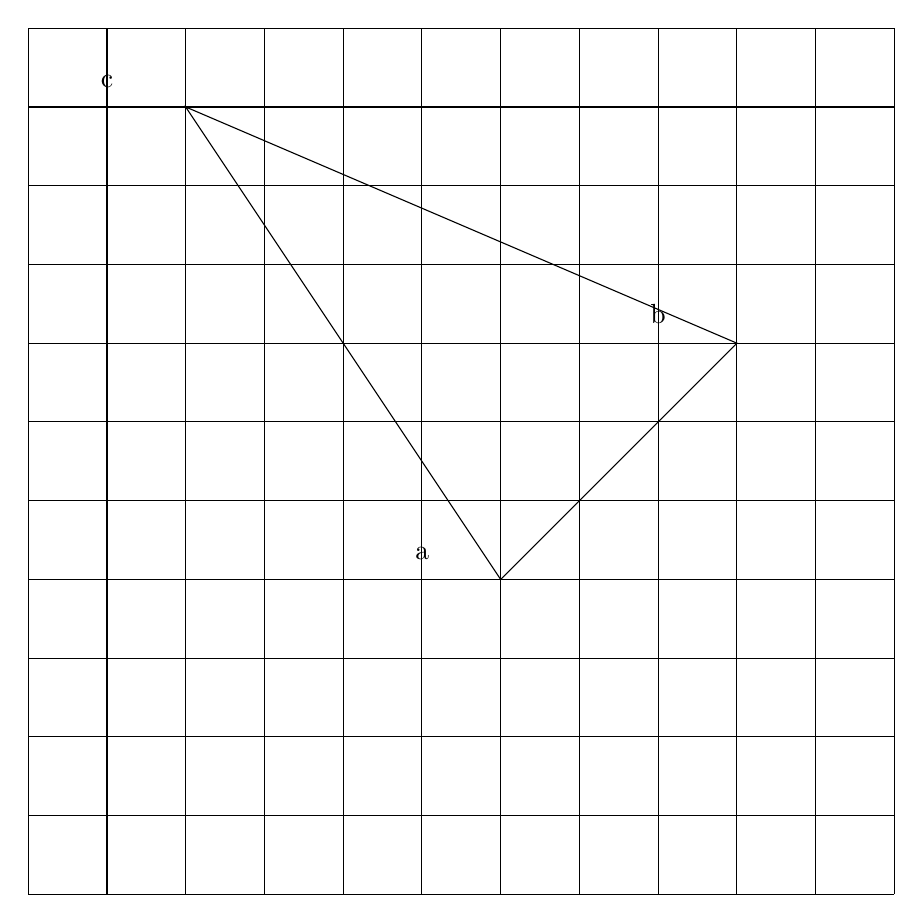
\begin{tikzpicture}
	\draw (-5, -5) grid (6, 6);
	
	\coordinate (a) at (1, -1);
	\coordinate (b) at (4, 2);
	\coordinate (c) at (-3, 5);
	
	\node[label=above:a, left of=a](a){};
	
	\node[label=above:b, left of=b](b){};
	\node[label=above:c, left of=c](c){};
	
	\draw (1, -1) -- (4, 2) -- (-3, 5) -- cycle;
\end{tikzpicture}

b) $(5, -2)(-2, -4), (1, 4)$

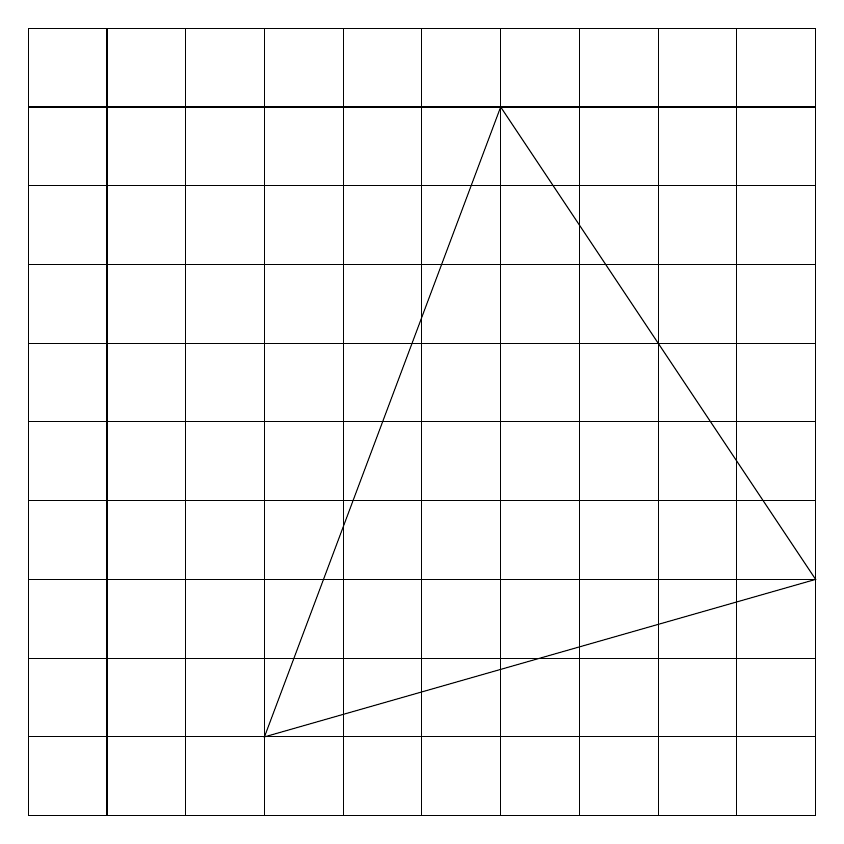
\begin{tikzpicture}
\draw (-5, -5) grid (5, 5);

\coordinate (a) at (5, -2);
\coordinate (b) at (-2, -4);
\coordinate (c) at (1, 4);

\draw (a) -- (b) -- (c) -- cycle;


\end{tikzpicture}


\subsubsection{10}

Find the length of the sides and the hypotenuse of the right triangle whos vertices are;

a) (1, 2), (-3, 2), (-3, 5)

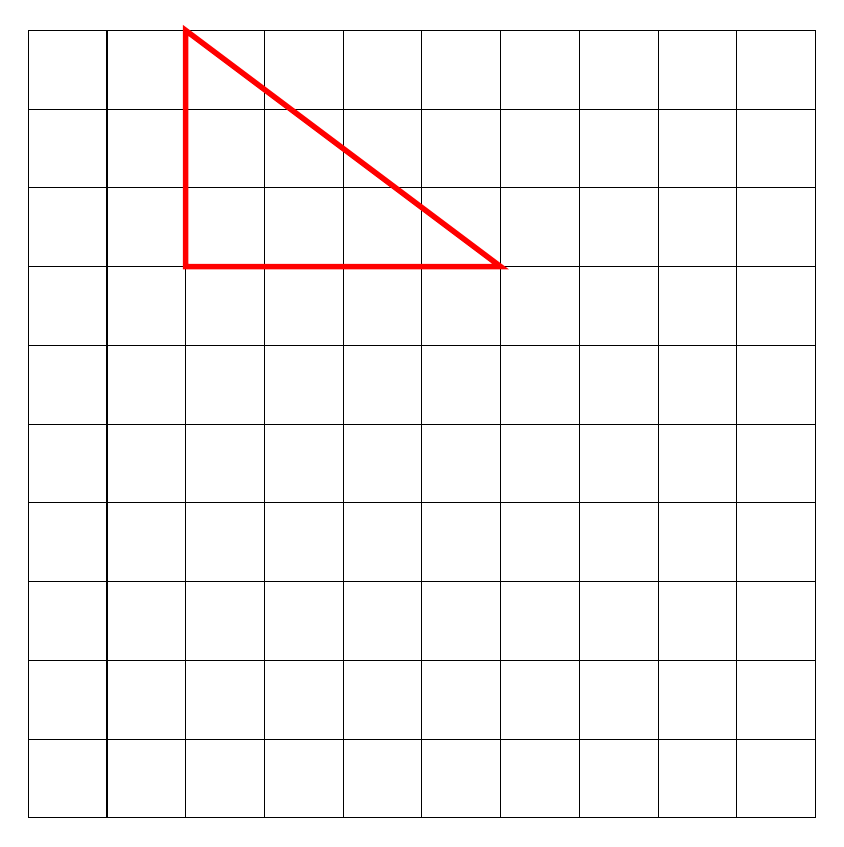
\begin{tikzpicture}
\draw (-5, -5) grid (5, 5);

\coordinate (a) at (1, 2);
\coordinate (b) at (-3, 2);
\coordinate (c) at (-3, 5);

\draw [line width=2pt, red] (a) -- (b) -- (c) -- cycle;

\end{tikzpicture}

\[
height = 3, base = 4, hypotenuse = \sqrt{3^2 + 4^2} = \sqrt{9 + 16} = \sqrt{25} = 5
\]

b) (2, -5), (2, 7), (-3, 7)

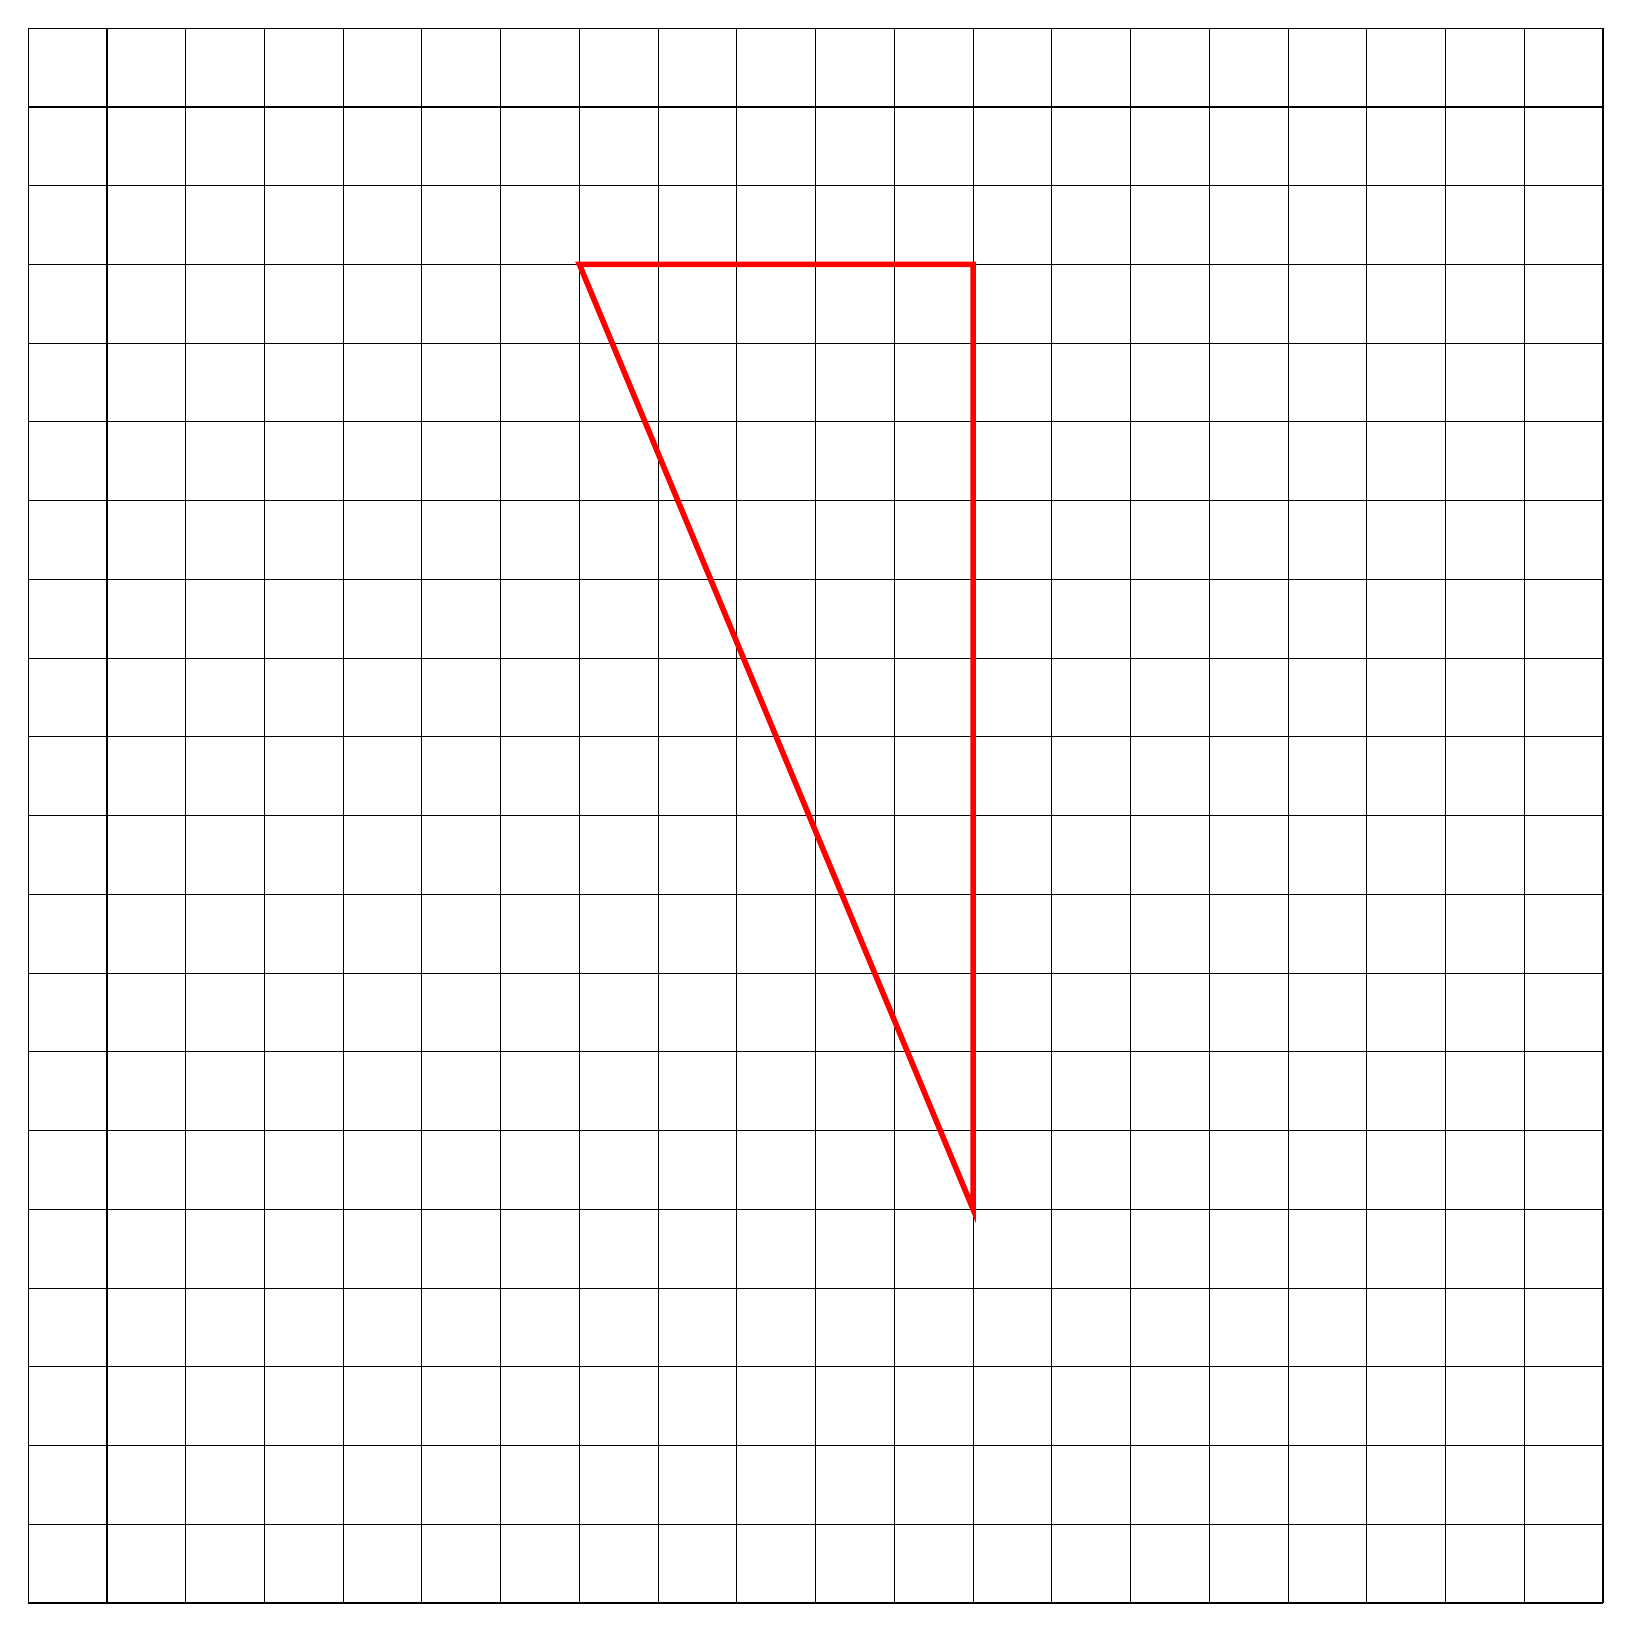
\begin{tikzpicture}
\draw (-10, -10) grid (10, 10);

\coordinate (a) at (2, -5);
\coordinate (b) at (2, 7);
\coordinate (c) at (-3, 7);

\draw [line width=2pt, red] (a) -- (b) -- (c) -- cycle;
\end{tikzpicture}

\[
height = 12, base = 5, hypotenuse = \sqrt{5^2 + 12^2} = \sqrt{25+ 144} = \sqrt{169} = 13
\]

\subsubsection{11}

Find the area of the rectangle whoose vertices are

a) $(4, 1), (-2, 3), (-2, 1), (4, 3) $


\begin{tikzpicture}
\draw (-5, -5) grid (5, 5);
\coordinate (a) at (4, 1);
\coordinate (b) at (-2, 3);
\coordinate (c) at (-2, 1);
\coordinate (d) at (4, 3);

\draw[line width=3pt, red] (a) -- (d) -- (b) -- (c) -- cycle;


\end{tikzpicture}

\[
height =  3 - 1 = 2, width = 4 - (-2) = 6, area = 2 \cdot 6 = 12
\]


b) $(-3, 7), (4, 2), (-3, 2), (4, 7) $


\begin{tikzpicture}
\draw (-8, -8) grid (8, 8);

\coordinate (a) at (-3, 7);
\coordinate (b) at (4, 2);
\coordinate (c) at (-3, 2);
\coordinate (d) at (4, 7);

\draw[line width=3pt, red] (a) -- (d) -- (b) -- (c) -- cycle;

\end{tikzpicture}

\[
height = 7 - 2 =  5, width  = 4 - (-3) = 7, area = 5 \cdot 7 = 35
\]


\subsubsection{12}
Find the coordinates of the midpoint of the segment joining

a) $(0, 0) to (6, 8)$

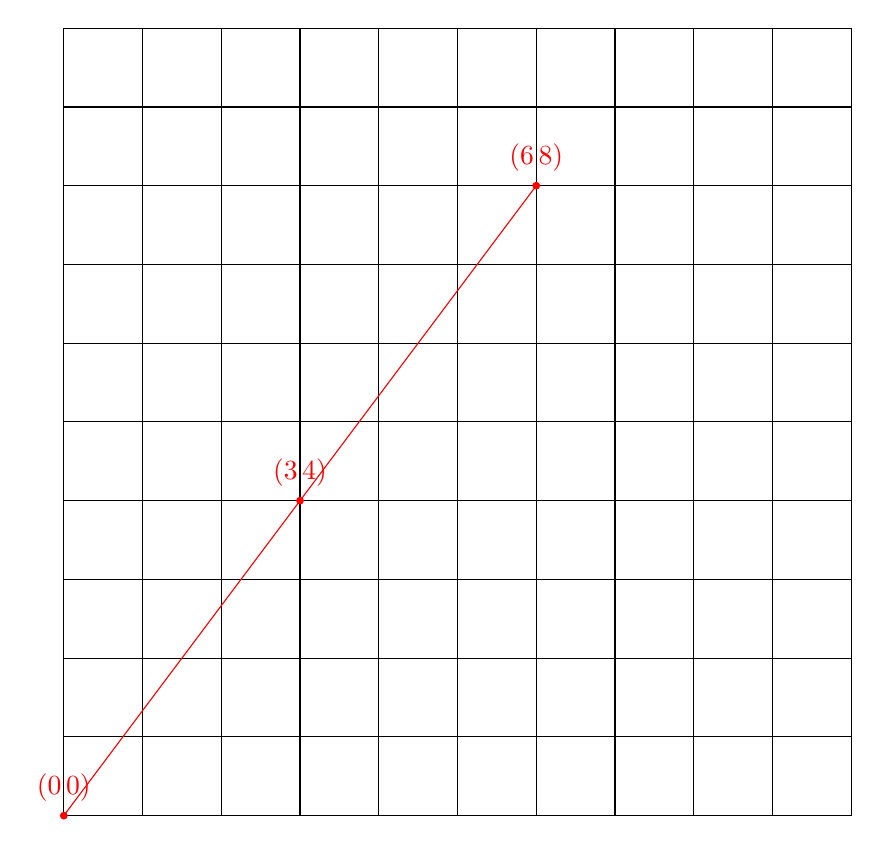
\begin{tikzpicture}
\draw (0, 0) grid (10,10);

\draw[red] (0, 0)  node[circle, fill, inner sep=1pt, label=above:(0\,0)](a){} -- (6, 8) node[circle, fill, inner sep=1pt, label=above:(6\,8)](b){};

\draw[red] (3, 4)  node[circle, fill, inner sep=1pt, label=above:(3\,4)](mid){};

\end{tikzpicture}



\[
midpoint = (0 + \frac{6-0}{2}, 0 + \frac{8-0}{2}) = (3, 4)
\]

b) $(1, 2) to (7, 8)$

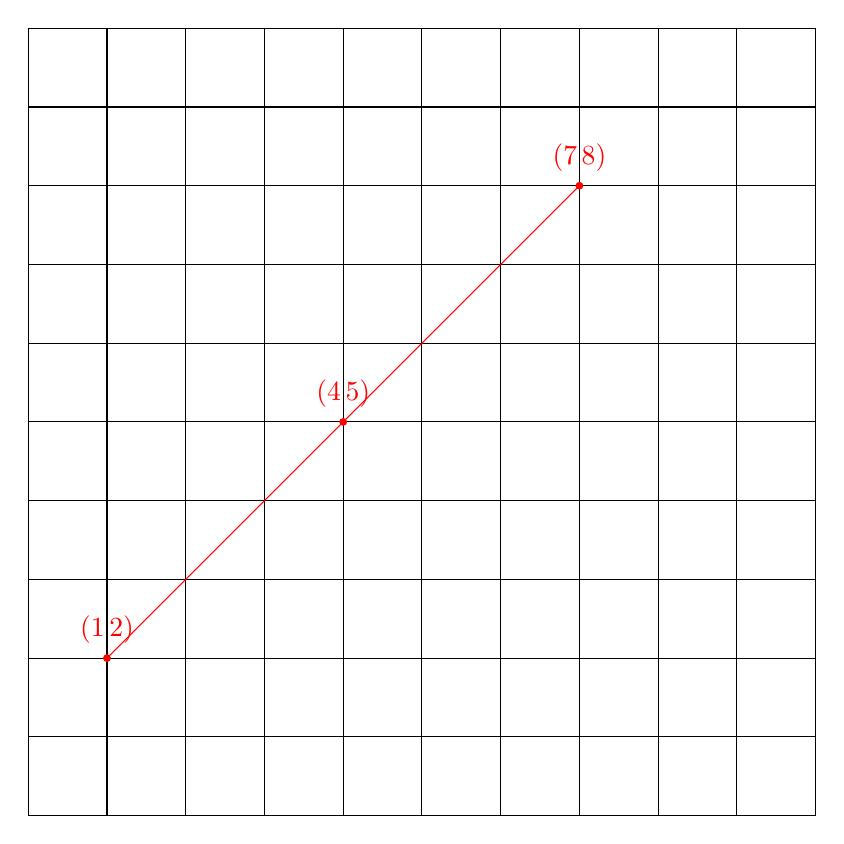
\begin{tikzpicture}
\draw (0, 0) grid (10, 10);

\draw[red] (1, 2) node[circle, fill, inner sep=1pt, label=above:(1\,2)](a){} -- (7, 8) node[circle, fill, inner sep=1pt, label=above:(7\,8)](b){};

\draw[red] (4, 5)  node[circle, fill, inner sep=1pt, label=above:(4\,5)](mid){};
\end{tikzpicture}

\[
midpoint = (1 + \frac{7 - 1}{2}, 2 + \frac{8 - 2}{2}) = (4, 5)
\]

\subsubsection{13}

Sketch on a suitable diagram all points (x, y)
such that

a) $x = 3$


\begin{tikzpicture}
\draw (0, 0) grid (5, 5);

\draw [red] (3, 0) -- (3, 5);

\end{tikzpicture}

b) $y= -4$


\begin{tikzpicture}
\draw (-5, -5) grid (5, 5);

\draw [red] (-5, -4) -- (5, -4);
\end{tikzpicture}

c) $x<3 and y > 2$


\begin{tikzpicture}
\draw (-5, -5) grid (5, 5);

\draw [red, fill] (-5, 3) -- (2, 3) -- (2, 5) -- (-5, 5) -- cycle;
\end{tikzpicture}

d) x or y (or both) is zero


\begin{tikzpicture}
\draw (-5, -5) grid (5, 5);

\draw [red] (0, 0) -- (5, 0);

\draw [red] (0, 0) -- (0, 5);

\end{tikzpicture}

e) $x >= 0 $ and $y <= 0$

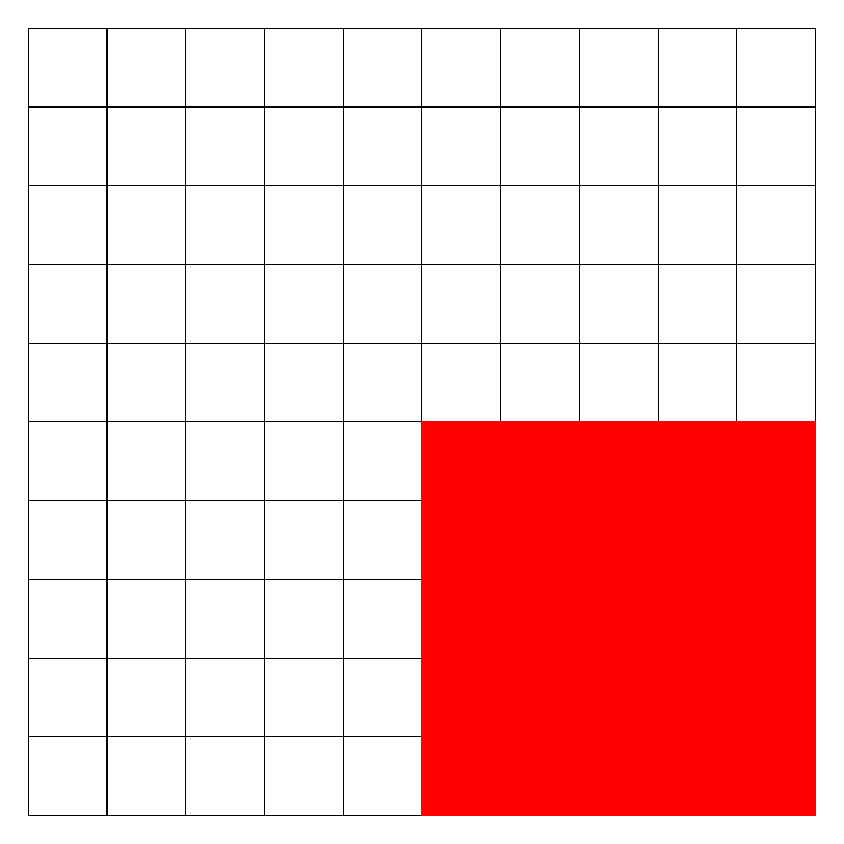
\begin{tikzpicture}
\draw(-5, -5) grid (5, 5);

\draw [red, fill] (0, 0) -- (0, -5) -- (5, -5) -- (5, 0) -- cycle;
\end{tikzpicture}


f) $x^2 <= 1$

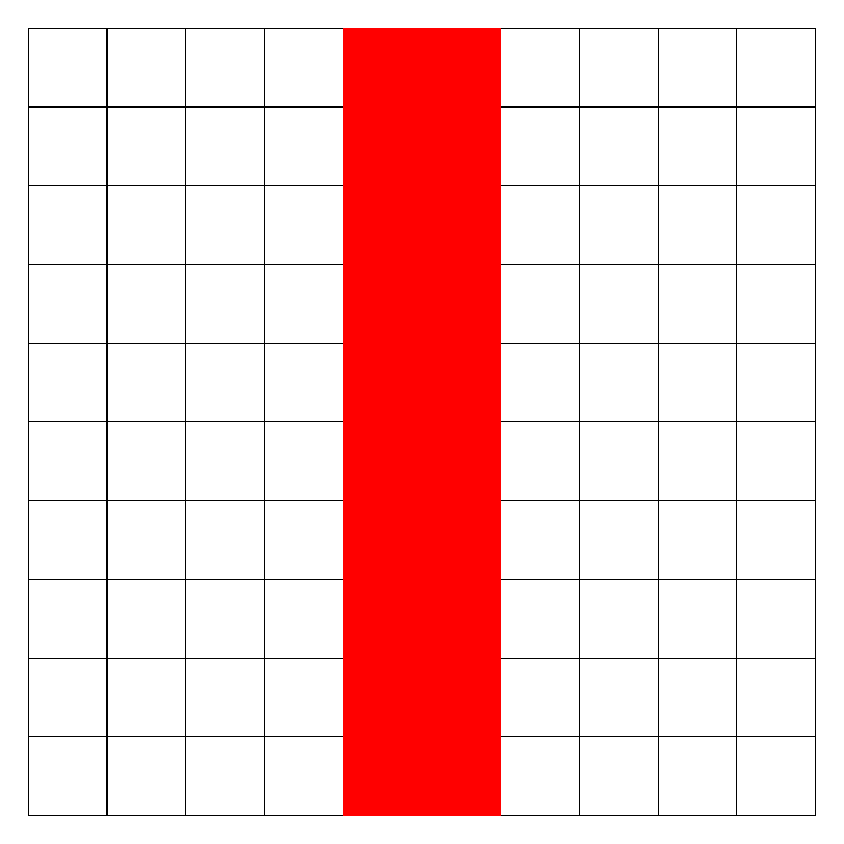
\begin{tikzpicture}
	\draw (-5, -5) grid (5, 5);
	
	\draw [red, fill] (-1, -5) -- (1, -5) -- (1, 5) -- (-1, 5) -- cycle;
\end{tikzpicture}


\subsubsection{14}

Find the slope determined by 

a) $(1, 2)$ and $(3, 6)$

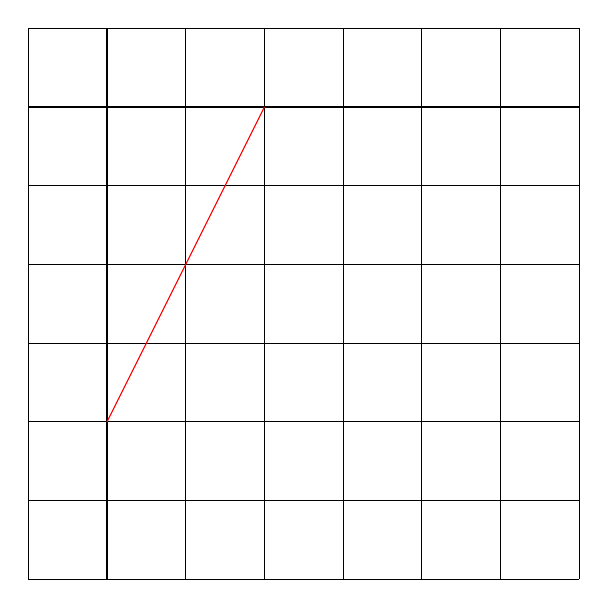
\begin{tikzpicture}
\draw(0, 0) grid (7, 7);

\draw [red](1, 2) -- (3, 6);
\end{tikzpicture}

\[
	m = \frac{6 - 2}{3 - 1} = \frac{4}{2} = 2
\]

b) $(-2, 4)$ and $(3, 4)$


\begin{tikzpicture}
\draw (-5,-5 ) grid (5, 5);

\draw [red] (-2, 4) -- (3, 4);
\end{tikzpicture}

\[
m = \frac{3 - (-2)}{4-4} = 0
\]

c) $(-2, 1)$ and $(2, -3)$

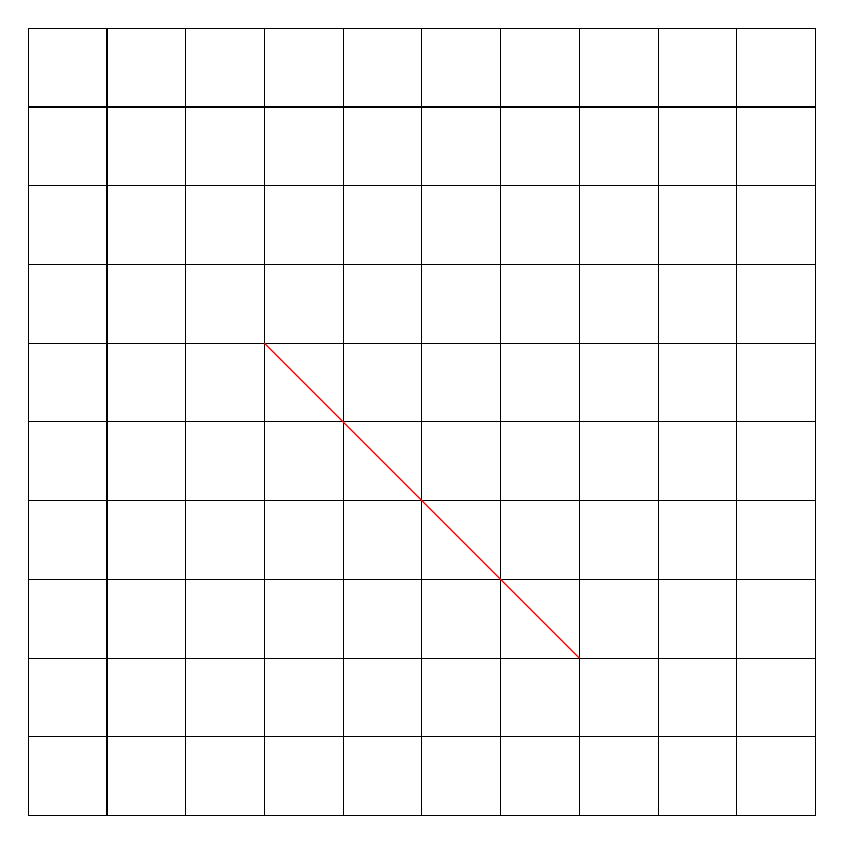
\begin{tikzpicture}
\draw(-5, -5) grid (5, 5);

\draw [red] (-2, 1) -- (2, -3);
\end{tikzpicture}

\[
	m = \frac{-3 - 1}{2 - (-2)} = \frac{-4}{4} = -1 
\]


\subsubsection{15}

Find the equation of the line through

a) $(-1, -2)$ and $(1, 0)$

\[
m = \frac{0 - (-2)}{1 - (-1)} = \frac{2}{2} = 1; 0 = 1 \cdot 1 + c; c = -1; y = x - 1
\]

b) $(0, 4)$ and $(1, 7)$

\[
m = \frac{7 - 4}{1 - 0} = \frac{3}{1} = 3; c = 7 - 3\cdot 1 = 4; y = 3x + 4
\]

c) $(4, -2)$ and $(4, 19)$

\[
m = \frac{19 - (-2)}{4 - 4} = 0; x = 4
\]


\subsubsection{16}

Show that the lines $3x + y = 2$ and $2y = 1- 6x$ are parallel

\begin{align*}
3x + y = 2 \tag{Equation 1}\\
y = -3x + 2 \tag{when rearranged}\\
\\
2y = 1 - 6x \tag{Equation 2}	\\
y = \frac{1 - 6x}{2} = \frac{1}{2} - 3x \tag{when rearranged}
\end{align*}

Given Equation 1 and Equation 2 have same slope, they will never intercept unless they are the same line, but given the y intercepts are different, then they aren't the same line. Meaning the cross the y axis at different points and slope in same direction


\subsubsection{17}

Write the equation of the line through (-2, -3) which is 

a) parallel to $x + 2y = 3$

Rearranging, we get $y = \frac{3 - x}{2}$

For the line to be parallel, the slope will be the same, thus $m=\frac{1}{2}$ The y intercept $c$ will be $-3 = \frac{1}{2}\cdot -2 + c; c=-2$

\[
	y = \frac{1}{2}x -2
\]

b) perpendicular to $x + 2y = 3$

Rearranging, we get $y = \frac{3 - x}{2}$

For the line to be perpendicular, the slope will now be different. Lets call the slope of the original equation, $m_1$ and the slope of the perpendicular equation, $m_2$. And that two slopes being perpendicular satisfy $m_1\cdot m_2 = -1$

Thus the slope of the perpendicular line, is $-\frac{1}{2}m_2 = -1$ or $m_2 = 2$

now for the point $(-2, -3)$ we have $ -3 = 2 \cdot (-2) + c$ or $c = 1$

So the perpendicular line is

$y = 2x + 1$


\subsubsection{18}

Write the equation of the circle with

a) center (0,0) and radius 2;

$ (x + 0)^2 + (y+0)^2 = x^2 + y^2 = 2^2$


b) center (-2,0) and radius 7;

$(x+2)^2 +y^2 = 49$

c) center (3,6) and radius $\frac{1}{2}$;

$(x-3)^2 + (y-6)^2 = \frac{1}{4}$

d) with (5, 5) and (-3, -1) as the ends of a diameter

Proposing we draw a straight line from $(5, 5)$ to $(-3, -1)$, the midpoint indicates the center.
$(\frac{5-3}{2}, \frac{5-1}{2}) = (1, 2)$

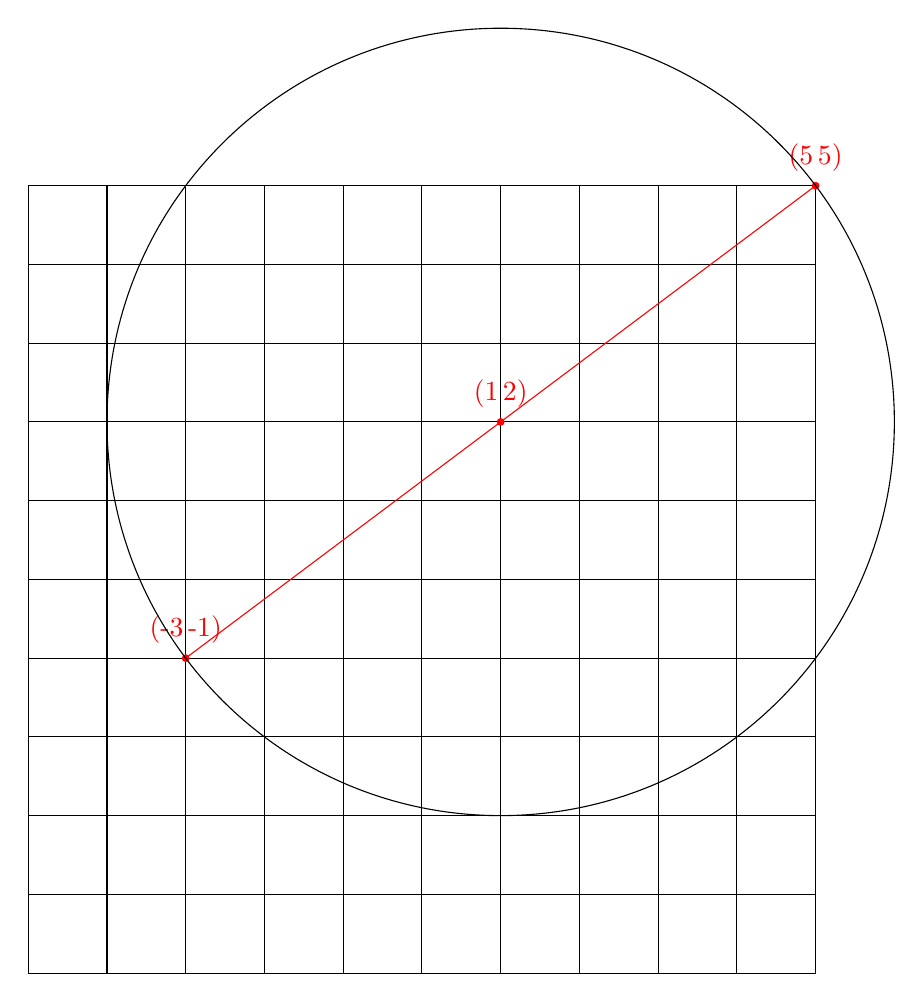
\begin{tikzpicture}
\draw (-5, -5) grid (5, 5);


\draw[red] (-3, -1)  node[circle, fill, inner sep=1pt, label=above:(-3\,-1)](a){} -- (5, 5) node[circle, fill, inner sep=1pt, label=above:(5\,5)](b){};

\draw[red] (1, 2)  node[circle, fill, inner sep=1pt, label=above:(1\,2)](mid){};

\draw (1, 2) circle (5);

\end{tikzpicture}

thus the equation of the ciircle is 

\[
(x-1)^2 + (y-2)^2 = 25
\]

\subsubsection{19}

Find the center and radius of the circle whose equation is

a) $(x + 3)^2 + (y - 6) ^2 = 9$

$r = \sqrt{9} = 3$

$center = (-3, +6)$


b) $(x - 4)^2 + (y) ^2 = 4$

$r = 2$

$center = (4, 0)$


c) $(x )^2 + (y + 2) ^2 = 1$

$r = 1$

$center = (0, -2)$


d) $x^2 + y^2 + 6x + 2y + 6  = 0$
\begin{align*}
	x^2 + y^2 + 6x + 2y + 6  = 0 \tag{1} \\
	(x + 3)^2 + (y+1)^2  -4 = 0  \tag{factoring out x and y} \\
	(x + 3)^2 + (y+1)^2 = 4
\end{align*}

Thus, $radius = \sqrt{4} = 2$ and $center = (-3, -1)$

e) $x^2 + y^2 - 16x + 14y + 97 = 0$

\begin{align*}
x^2 + y^2 - 16x + 14y + 97 = 0	\tag{1} \\
x^2 - 16x + 48 + (y + 7)^2 = 0 \tag{factoring out y}\\
(x-8)^2 + (y+7)^2 - 16 = 0 \tag{factoring out x} \\
(x-8)^2 + (y+7)^2 = 16
\end{align*}

Thus $radius = \sqrt{16} = 4$ and center $(8, -7)$

\subsubsection{20}

On a single set of coordinate axes, sketch the line $x + 16 = 7y$ and the circle $x^2 + y^2 - 4x + 2y = 20$ and find their points of intersection.

\begin{align*}
	x + 16 = 7y \tag{1} \\
	x = 7y - 16 \tag{rearranging} \\
	x^2 + y^2 - 4x + 2y = 20  \tag{2} \\
	(7y - 16)^2 + y^2 - 4(7y -16) + 2y = 20 \tag{eliminating x} \\
	49y^2 - 224y + 256 + y^2 - 28y  + 64 + 2y = 20 \tag{expanding} \\
	50y^2 - 250y + 320 = 20 \\
	50y^2 - 250y + 300 = 0 \\
	y = \frac{250 \pm \sqrt{(-250)^2 - 4 \cdot 50 \cdot 300}}{2 \cdot 50} \\
	y = \frac{250 \pm \sqrt{2500}}{100} = \frac{250 \pm 50}{100}\\
	y = \frac{200}{100} = 2, or, y = \frac{300}{100} = 3
\end{align*}

Thus, when $y = 2$, $x = 7\cdot 2 - 16 = -2$ and when $y = 3$ then $x = 7\cdot 3 -16 = 5$

So the points on intersection are, (-2, 2) and (5, 3)


\subsubsection{21}
Find the focus and directrix of each of the following parabolas

a) $ y = 2x^2$

So as $ y = 2x^2$, this will have points on the parabola where $ y >= 0$, so looking like 

\begin{tikzpicture}
\begin{axis}[
domain=-1:1,
samples=101,
smooth,
no markers,
]
\addplot {2*x^2};
\end{axis}
\end{tikzpicture}

That means the minimum/vertex of this parabola will be (0, 0)

This means that the directrix must be when $ y < 0 $ and the value $y = 0$ is halfway between the directrix's y value and the focus' y value. Lets (using the notation from the book) define $p$ as the value indicating this scalar distance, where the directrix is $y = -p$ and the focus be located at $(0, p)$ and the parabola as the equation $y = \frac{1}{4p}x^2$

Thus we have

\begin{align*}
\frac{1}{4p} = 2\\
1 = 2 \cdot 4p = 8p\\
p = \frac{1}{8}
\end{align*}

So the focus $(0, \frac{1}{8})$ and directrix $y = - \frac{1}{8}$





b) $y = \frac{1}{8}x^2$

\begin{tikzpicture}
\begin{axis}[
domain=-1:1,
samples=101,
smooth,
no markers,
]
\addplot {(1/8)*x^2};
\end{axis}
\end{tikzpicture}

Vertex: (0, 0);
focus = $\frac{1}{4p} = \frac{1}{8}; 4p = 8; p=2, (0, 2)$
directrix = $-2$

c) $y = -5x^2$

\begin{tikzpicture}
\begin{axis}[smooth, no markers]
\plot {-5 * x^2};
\end{axis}
\end{tikzpicture}

\[
-\frac{1}{4p} = -5; -1 = -20p; p=\frac{1}{20}
\]

So focus this time is when $y < 0$

Focus = $(0, -\frac{1}{20})$

Directrix = $y = \frac{1}{20}$

d) $y = -\frac{1}{12}x^2$

\begin{tikzpicture}
\begin{axis}[smooth, no markers]
\addplot {-(1/12) * x^2};
\end{axis}
\end{tikzpicture}

\[
-\frac{1}{4p} = -\frac{1}{12}; -4p = -12; p = 3;
\]

Focus = (0, -3)

Directrix $y = 3$

\subsubsection{22}

A parabola has vetical axis and vertex at the origin.

Write its equation if its focus is at 

a) $(0, 3)$

So given the vertex is at the origin, and this has value of $p = 3$

$ y = \frac{1}{4p}x^2 = \frac{1}{4\cdot3}x^2 = \frac{1}{12}x^2$

b) $(0, 16)$

$y = \frac{1}{64}x^2$

c) $(0, -1)$

$ p = -1$

$ y = \frac{1}{4p}x^2 = \frac{1}{4\cdot (-1)} x^2 = -\frac{1}{4}x^2$

d) $(0, -\frac{1}{10})$

$p = -\frac{1}{10}$

$y = \frac{1}{4 \cdot -\frac{1}{10}}x^2 = \frac{1}{-\frac{4}{10}}x^2 = -\frac{10}{4}x^2 = -\frac{5}{2}x^2$


\subsubsection{23}

Find the vertex and focus of each of the following parabolas, and state whether it opens up or down;

a) $y = x^2 - 4x + 1$

\begin{align*}
y = x^2 -4x + 1 \tag{1} \\
y - 1 = x^2 -4x \tag{taking 1 off both sides} \\
y -1 = (x-2)^2 - 4 \tag{completing the square} \\
y + 3 = (x-2)^2 \\
\bar{y} = (y+3)  \tag{Assigning the left hand side to a new y coordinate system}\\
\bar{x} = (x-2) \tag{Similarly for the right hand side to a new x coordinate system}\\
\bar{y} = \bar{x}^2
\end{align*}

$\bar{y} = \frac{1}{4p}\bar{x}^2 = \frac{1}{4 \cdot \frac{1}{4}}\bar{x}^2$

So on the equation $\bar{y} = \bar{x}^2$, $p = \frac{1}{4}$ meaning Focus on this is $(0, \frac{1}{4})$ and Directrix is $y = -\frac{1}{4}$

Translating this back to the old coordinate system

The vertex is $(2,-3)$

and the focus is $(2, -2\frac{3}{4})$

\begin{tikzpicture}
\begin{axis}[smooth, no markers]
\addplot {x^2 - 4*x + 1};
\end{axis}
\end{tikzpicture}

b) $y = 2x^2 - 12x - 7 $

\begin{align*}
y = 2x^2 - 12x - 7  \tag{1} \\
y = 2(x^2 - 6x - \frac{7}{2}) \\
y = 2((x - 3)^2 -9 - \frac{7}{2}) \\
y = 2((x- 3)^2 - \frac{25}{2}) \\
y = 2(x-3)^2 - 25\\
y + 25 = 2(x-3)^2
\end{align*}

$\frac{1}{4p} = 2$
So

$\frac{1}{4} = 2p$ or $p = \frac{1}{8}$

Vertex (3, -25)

Focus $(3, -24\frac{7}{8})$

up

\begin{tikzpicture}
\begin{axis}[smooth, no markers]
\addplot {2*x^2 - 12*x -7};
\end{axis}
\end{tikzpicture}

c) $y = -x^2 -4x + 5$

\begin{align*}
y = -x^2 -4x + 5 \tag{1} \\
y = -1 (x^2 + 4x - 5) \tag{pulling the negative 1 out} \\
y = -1 ((x + 2)^2 -4  -5) \tag{factoring and completing the square} \\
y = -1(x+2)^2 + 9 \\
(y-9) = -1(x+2)^2 \\
\bar(y) = y-9 \\
\bar{x} = x+2
\end{align*}
$\bar{y} = -1\bar{x}^2$

$\frac{1}{4p}  = -1$

$-p = \frac{1}{4}$ or $p = -\frac{1}{4}$

Vertex (-2, 9)

Focus $(-2,  8\frac{3}{4})$

\begin{tikzpicture}
\begin{axis}[smooth, no markers]
\addplot{-1 * x^2 - 4*x + 5};
\end{axis}
\end{tikzpicture}

d) $y = 4 - 2x - \frac{1}{2} x^2$

\begin{align*}
y = 4 - 2x - \frac{1}{2} x^2 \tag{1} \\
y = -\frac{1}{2}(-8 + 4x + x^2) \\
y = -\frac{1}{2}(-8 + (2 + x)^2 - 4) \tag{completing the square} \\
y = -\frac{1}{2}(-12 + (2 + x)^2) \\
y = 6 -\frac{1}{2}((2 + x)^2)\\
y - 6 = -\frac{1}{2}((2 + x)^2)
\end{align*}

$\frac{1}{4p} = -\frac{1}{2}$
$2 = -4p$ so $p = -\frac{1}{2}$

Vertex (-2, 6)

Focus $(-2, 5\frac{1}{2})$

Down

\begin{tikzpicture}
\begin{axis}[smooth, no markers]
\addplot{4 - 2*x - 0.5 * x^2};
\end{axis}
\end{tikzpicture}

\subsubsection{24}
Without actually finding the roots, determine for each equation whether its roots are; real and distinct, real and equal, or imaginary.

Using the formula $b^2 - 4ac$ to determine if the roots are real and distinct, real and equal, or real and imaginary,

where real and distinct $b^2 - 4ac > 0$
where real and equal $b^2 - 4ac = 0$
and imaginary $b^2 - 4ac < 0$

a) $5x^2 +3x + 4 = 0$

\[
3^2 - 4\cdot5\cdot4 = 9 - 80 = -71
\]

Imaginary

b) $7x^2 -2x - 15 = 0$

\[
-2^2 - 4\cdot7\cdot(-15)  = 4 + 420
\]

Real and distinct

c) $3x^2 -5x +1 = 0$

\[
-5^2 - 4\cdot3\cdot1 = 25 -12 = 13
\]

Real and distinct

d) $4x^2 + 20x + 25 = 0$

\[
20^2 - 4\cdot4\cdot25 = 400 - 400 = 0
\]

Real and unique

\subsubsection{25}
Without solving, find the sum and product of the roots 

Sum of roots $-\frac{b}{a}$

Product of roots $\frac{c}{a}$

a) $4x^2 - 7x -13 = 0$
Sum; $-\frac{7}{4}$
Product = $-\frac{13}{4}$

b) $3x^2 + 10x + 17 = 0$
Sum; $-\frac{10}{3}$
Product; $\frac{17}{3}$


c) $2x^2 + x - 2 = 0$
Sum; $-\frac{1}{2}$
Product -1

\subsubsection{26}

Construct a quadratiuc equation having the given numbers as roots

a) -3, 8

Sum of roots = 5  = $-\frac{b}{a}$

Product of roots = -24 = $\frac{c}{a}$

Letting a=1, b = -5, c = -24

$x^2- 5x -24 = 0$

b) $2 + \sqrt{5}, 2 - \sqrt{5}$

Sum of roots = $4 = -\frac{b}{a}$

Product of roots = $-1 = \frac{c}{a}$

Letting a=1, b = -4, c = -1

$x^2 - 4x -1 = 0$

c) $-\frac{3}{5}, \frac{2}{3}$

Sum of roots = $ \frac{-9 + 10}{15} = \frac{1}{15} = -\frac{b}{a}$

Product of roots = $-\frac{6}{15}$

$15x^2 - x - 6 = 0$

\subsubsection{27}

Sketch the graph of $ y = f(x)$ if $f(x)$ equals

a) $x^2 -4x + 4$

\begin{tikzpicture}
\begin{axis}[smooth, no markers]
\addplot{x^2 - (4*x) + 4};
\end{axis}
\end{tikzpicture}

b) $x^2 - x - 2$

\begin{tikzpicture}
\begin{axis}[smooth, no markers]
\addplot{x^2 - x -2};
\end{axis}
\end{tikzpicture}

c) $\frac{1}{x^2}$


\begin{tikzpicture}
\begin{axis}[smooth, no markers]
\addplot{1/(x^2)};
\end{axis}
\end{tikzpicture}

d) $\frac{x}{x^2 + 1}$

\begin{tikzpicture}
\begin{axis}[smooth, no markers]
\addplot{x/(x^2+1};
\end{axis}
\end{tikzpicture}


\subsection{3 - Special Topics}

\subsubsection{1}

Express each of the following in terms of logarithms;

a) $5^2 = 25$

\[
2 = \log_5 {25}
\]

b) $2^5  = 32$

\[
5 = \log_2 32
\]

c) $5^{-2} = \frac{1}{25}$

\[
-2 = \log_5 \frac{1}{25}
\]

d) $2^6 = 64$

\[
6 = \log_2 64
\]

e) $3^3 = 27$

\[
3 = \log_3 27
\]

f) $81^{0.5} = 9$

\[
0.5 = \log_{81} 9
\]

g) $7^0 =1$

\[
0 = \log_7 1
\]

h) $10^{-1} = \frac{1}{10}$

\[
-1 = \log_{10} \frac{1}{10}
\]

i) $32^{\frac{4}{5}} = 16$

\[
\frac{4}{5} = \log_{32} 16
\]

j) $16^{0.75} = 8$

\[
0.75 = \log_{16} 8
\]

\subsubsection{2}

a)

\[
10^1 = 10
\]

b)

\[
8 = 4^{\frac{3}{2}}
\]


c)

\[
8 = 2^3
\]

d)

\[
\frac{1}{125} = 5^{-3}
\]

e)

\[
81 = 9^2
\]

f)

\[
1 = 10^0
\]

g)

\[
0.01 = 10^{-2}
\]

h) 

\[
343 = 7^3
\]

i)

\[
125 = 5^3
\]

j)

\[
0.1 = 10^{-1}
\]

\subsubsection{3}

a) $\log_2 2 = 1$

b) $\log_{10} 10000 = 4$

c) $\log_2 16 = 4$

d) $\log_{25} 125 = \frac{3}{2}$

e) $\log_{10} 0.001 = -3$

f) $\log_8 4 = \frac{2}{3}$

g) $\log_2 1 = 0$

h) $\log_8 \frac{\sqrt{2} \cdot \sqrt[3]{256}}{\sqrt[6]{32}}$ TODO

i) TODO


\subsubsection{4}

Solve for x

a) $\log_9 x = 3.5$ so x = 2187

b) $\log_{27} x = \frac{5}{3}$ so x 243

c) $\log_2 x = 8 $ so x 256

d) $\log_{32}x = 0.8$ so x is 16

\subsubsection{5}

Find the base a

a) $\log_a 9 = 0.4$ so a = 243

b) $\log_a 27 = -\frac{3}{4}$ a = $\frac{1}{81}$

c) $\log_a 49 = 2$ so a = 7

d) $\log_a 6 = \frac{1}{2}$ a = 36

\subsubsection{6}

TODO: Determine nicest formatting for long division

a) 
\begin{align*}
	x - 2\\
x-3 ) \overline{x^2 - 5x + 6}\\
- (x^2 -3x)\\
\overline{0x^2 -2x + 6} \\
- (-2x + 6)\\
\overline{0x^2 + 0x + 0}
\end{align*}

$Q(x) = x-2 $ and $R(x) = 0$

b)

\begin{align*}
x + 3\\
x-7) \overline{x^2 -4x -21}\\
- (x^2 - 7x)\\
\overline{3x - 21}\\
-(3x - 21)\\
\overline{0}
\end{align*}

$Q(x) = x + 3$ and $R(x) = 0$

c)

\begin{align*}
x^2 - x - 6\\
x-7 ) \overline{x^3 - 8x^2 + x + 42}\\
- (x^3 - 7x^2)\\
\overline{-x^2 + x + 42}\\
- (-x^2 + 7x)\\
\overline{-6x + 42}\\
- (-6x + 42) \\
\overline{0}
\end{align*}

$Q(x) = x^2 -x -6$ and $R(x) = 0$

d) 

\begin{align*}
3x^2 - 2x + 1\\
x^2 + 3) \overline{3x^4 - 2x^3 + 10x^2 -7x + 10}\\
-(3x^4 + 9x^2)\\
\overline{-2x^3 + x^2 -7x + 10} \\
-(-2x^3 - 6x)\\
\overline{x^2 - x + 10} \\
- (x^2 + 3) \\
\overline{-x + 7}
\end{align*}

$Q(x) = 3x^2 - 2x + 1$ and $R(x) = -x + 7$

e)

\begin{align*}
x^3 - 2x^2 + 5\\
x^2 -  2x - 1) \overline{x^5 - 4x^4 + 3x^3 + 7x^2 - 10x -5}\\
- (x^5 - 2x^4 - x^3)\\
\overline{-2x^4 +  4x^3 + 7x^2 - 10x - 5} \\
- (-2x^4 + 4x^3 + 2x^2)\\
\overline{5x^2 - 10x - 5}\\
- (5x^2 - 10x - 5)\\
\overline{0}
\end{align*}

$Q(x) = x^3 - 2x^2 + 5$ and $R(x) = 0$


\subsubsection{7}

Use the factor theorem to show that 

a) $x^91 + 3x^73 - 2x^37 -2$ has $x-1$ as a factor.

To test this, we will apply the value $x = 1$ to $x^91 + 3x^73 - 2x^37 -2 = 0$

\[
1^91 + 3(1)^73 - 2(x)^37 - 2 = 1 + 3 - 2 - 2 = 0
\]

So $x-1$ is a factor\\

b) $x^91 + x^74 + x^132 + x^51$ has $x+1$ as a factor

So given x = -1

\[
(-1)^91 + (-1)^74 + (-1)^132 + (-1)^51 = -1 + 1 + 1 - 1 = 0
\]

c) $x^5  - 3x^4 + 6x^3 - 5x^2 - 12$ has factor $(x-2)$

Given x = 2

\[
2^5 - 3(2)^4 + 6(2)^3 - 5(2)^2 - 12 = 32 - 48 + 48 -20 - 12 = 0
\]

\subsubsection{8}

\begin{align*}
x^{n-1} + x^{n-2} ...  + x + 1\\
x-1)\overline{x^n -1}\\
- (x^n - x^{n-1}) \\
\overline{x^{n-1} - 1}\\
...
\end{align*}

\subsubsection{9}

a) 

\begin{align*}
x^2  -5x + 6\\
x-1 ) \overline{x^3 - 6x^2 + 11x - 6}\\
- (x^3 -x^2)\\
\overline{-5x^2 + 11x - 6} \\
-(-5x^2 + 5x)\\
\overline{6x - 6}\\
-(6x -6) \\
\overline{0}
\end{align*}

Which means $(x-1)(x^2  -5x + 6) = 0 = (x-1)(x - 2)(x - 3)$

b)

\begin{align*}
x^2 + 1\\
x-1) \overline{x^3 -x^2 + x - 1}\\
-(x^3 -x^2)\\
\overline{x - 1}\\
- (x - 1)\\
\overline{0}
\end{align*}

Which means $(x-1)(x^2 + 1) = 0$

c)

\begin{align*}
x^2 + 3x - 18\\
x + 2) \overline{x^3 + 5x^2  - 12x -36}\\
- (x^3 +2x^2)\\
\overline{3x^2 - 12x -36}\\
-(3x^2 + 6x)\\
\overline{-18x - 36}\\
-(-18x - 36) \\
\overline{0}
\end{align*}

which means $(x+2)(x^2 + 3x - 18) = 0 = (x+2)(x+6)(x-3)$

d)

\begin{align*}
x^2 + 2x +  1\\
x-3) \overline{x^3 - x^2 - 5x - 3}\\
- (x^3 -3x^2)\\
\overline{2x^2 - 5x - 3}\\
- (2x^2 - 6x)\\
\overline{x - 3}\\
- (x - 3)\\
\overline{0}
\end{align*}

which means $(x-3)(x^2 + 2x + 1) = 0 = (x-3)(x+1)(x+1)$

\subsubsection{10}
a) 
$
\begin{vmatrix}
	1 & 2\\
	3 & 4
\end{vmatrix} = 4\cdot1 - 2\cdot3 = 4 -6 = -2
$

b) 
$
\begin{vmatrix}
-2 & 7 \\
-5 & -6
\end{vmatrix} = (-2) \cdot (-6) - (-5)\cdot 7 = 12 - (-35) = 47
$

\subsubsection{11}
determine
$
\begin{vmatrix}
+ & - & + \\
- & + & - \\
+ & - & +
\end{vmatrix}
$

a) $
\begin{vmatrix}
2 & 0 & -1 \\
3 & 2 & 6 \\
-4 & 5 & 0
\end{vmatrix}=
 2 \cdot \begin{vmatrix}
2 & 6\\
5 & 0
\end{vmatrix}
- 3\cdot \begin{vmatrix}
0 & -1\\
5 & 0
\end{vmatrix}
+ (-4)\cdot \begin{vmatrix}
0 & -1 \\
2&6
\end{vmatrix}
=2(-30) - 3(5) + (-4)(2) = -60 -15  - 8 = -83
$


b)$
\begin{vmatrix}
-2 & 4 & 6 \\
3 & 0 & 1 \\
1 & 1 & -7
\end{vmatrix}= - 3\cdot \begin{vmatrix}
4 & 6 \\
1 & -7
\end{vmatrix}
+ 0 \cdot \begin{vmatrix}
-2 & 6\\
1 & -7
\end{vmatrix}
- 1\cdot \begin{vmatrix}
-2 & 4\\
1 & 1
\end{vmatrix}= - 3(-28 - 6) + 0 - (-2 -4) = - 3(-34) - (-6) = - (-102) - (-6) = 108
$

\subsubsection{12}

Solve by determinants:

a)

$6x + 7y = 18$ \\
$9x - 2y = -48$

$x = \frac{
\begin{vmatrix}
18  & 7\\
-48 & -2
\end{vmatrix}
}{
\begin{vmatrix}
6 & 7 \\
9 & -2
\end{vmatrix}
} = \frac{-36 - (-336)}{-12 - 63} = \frac{-300}{-75} = -4$

$y = \frac{
	\begin{vmatrix}
	6  & 18\\
	9 & -48
	\end{vmatrix}
}{
	\begin{vmatrix}
	6 & 7 \\
	9 & -2
	\end{vmatrix}
} = \frac{-288 - 162}{-12 - 63} = \frac{-450}{-75} = 6$

To test, plugging in $6(-4) + 7(6) = 3(6) =  18$


b)

$2x + 3y + z = 4$ \\
$x + 5y - 2z = -1$ \\
$3x - 4y + 4z = -1$ \\

So we will be working with determinants of order 3,


$x = \frac{
\begin{vmatrix}
4 & 3 & 1\\
-1 & 5 & -2 \\
-1 & -4 & 4
\end{vmatrix}
}{
\begin{vmatrix}
2 & 3 & 1\\
1 &  5 & -2 \\
3 & -4 & 4
\end{vmatrix}
}$

For the denominator of $
\begin{vmatrix}
2 & 3 & 1\\
1 &  5 & -2 \\
3 & -4 & 4
\end{vmatrix} = 2 \cdot \begin{vmatrix}
5 & -2 \\
-4 & 4
\end{vmatrix} 
- 1 \cdot \begin{vmatrix}
3 & 1 \\
-4 & 4
\end{vmatrix}
+ 3 \cdot \begin{vmatrix}
3 & 1 \\
5 & -2
\end{vmatrix} = 2(20 - 8) - 1(12 - (-4)) + 3(-6 - 5) = 2(12) - 1(16) + 3(-11) = 24 - 16 - 33 = -25
$

And the numerator of $
\begin{vmatrix}
4 & 3 & 1\\
-1 & 5 & -2 \\
-1 & -4 & 4
\end{vmatrix} = 4 \cdot \begin{vmatrix}
5 & -2 \\
-4 & 4
\end{vmatrix}
- (-1)\cdot \begin{vmatrix}
3 & 1 \\
-4 & 4
\end{vmatrix}
+ (-1)\cdot \begin{vmatrix}
3 & 1 \\
5 & -2
\end{vmatrix} = 4(20 - 8) - (-1)(12 - (-4)) + (-1)(-6 - 5) = 4(12) - (-1)(16) + (-1)(-11) = 4(12) + 16 + 11 = 75
$

so $x = \frac{75}{-25} = -3$


$y = \frac{
	\begin{vmatrix}
	2 & 4 & 1\\
	1 & -1 & -2 \\
	3 & -1 & 4
	\end{vmatrix}
}{
	\begin{vmatrix}
	2 & 3 & 1\\
	1 &  5 & -2 \\
	3 & -4 & 4
	\end{vmatrix}
}$

Where the numerator is 

$	\begin{vmatrix}
2 & 4 & 1\\
1 & -1 & -2 \\
3 & -1 & 4
\end{vmatrix} = 2 \cdot \begin{vmatrix}
-1 & -2 \\
-1 & 4
\end{vmatrix}
- 1 \cdot \begin{vmatrix}
4 & 1\\
-1 & 4
\end{vmatrix}
+ 3 \cdot \begin{vmatrix}
4 & 1 \\
-1 & -2
\end{vmatrix}
= 2(-4 -2) - 1(16 - (-1)) + 3(-8 - (-1)) = 2(-6) - 1(17) + 3(-7) = -12 - 17 - 21 = -50 
$

$ y = \frac{-50}{-25} = 2$


$z = \frac{
	\begin{vmatrix}
	2 & 3 & 4\\
	1 & 5 & -1 \\
	3 & -4 & -1
	\end{vmatrix}
}{
	\begin{vmatrix}
	2 & 3 & 1\\
	1 &  5 & -2 \\
	3 & -4 & 4
	\end{vmatrix}
}$

Numerator
$	\begin{vmatrix}
2 & 3 & 4\\
1 & 5 & -1 \\
3 & -4 & -1
\end{vmatrix} = 2 \cdot \begin{vmatrix}
5 & -1 \\
-4 & -1
\end{vmatrix}
-1 \cdot \begin{vmatrix}
3 & 4 \\
-4 & -1
\end{vmatrix}
+ 3 \cdot \begin{vmatrix}
3 & 4 \\
5 & -1
\end{vmatrix}
= 2 (-5 - 4) - 1(-3 - (-16)) + 3(-3 - 20) = 2(-9) - (13) + 3(-23) = -18 - 13 - 69 = -100
$

$z = \frac{-100}{-25} = 4$


Plugging these into equation (1) we get
$2(-3) + 3(2) + 4 = -6 + 6 + 4 = 4$


\subsubsection{13}

If 5 bacteria enter a hunan body at the same time, and if each divides in two every 12 hours and non die, how many will there by a week later?

\[
NumberOfBacteria_{day1} = (5\cdot 2 \cdot 2) = 5 \cdot 2^{(2*1)}
\]

\[
NumberOfBacteria_{day2} = (5 \cdot 2 \cdot 2 \cdot 2 \cdot 2) = (5 \cdot 2^4) = 5 \cdot 2^{(2*2)}
\]

\[
NumberOfBacteria_{day3} = (5 \cdot 2 \cdot 2 \cdot 2 \cdot 2 \cdot 2 \cdot 2) = (5 \cdot 2^6)= 5 \cdot 2^{(2*3)}
\]

\[
NumberOfBacteria_{day n} = 5 \cdot 2^{(2*n)}
\]

\[
NumberOfBacteria_{day 7} = 5 \cdot 2^{14} = 81920
\]

\subsubsection{14}

$S = \frac{a(1 - r^{n+1})}{1-r}$

A golf ball is dropped from a height of 81 inches. If it always rebounds $\frac{2}{3}$ of the distance it falls, use formula (3) to find the total distance it has traveled if it is caught at the top of the fourth bounce.


$S = \frac{81(1 - \frac{2}{3}^{3+1})}{1-\frac{2}{3}} = \frac{81(1 - \frac{2}{3}^4)}{\frac{1}{3}} = 3 \cdot 81(1 - \frac{16}{81}) = 243 (\frac{65}{81}) = 195 $ inches downwards

Now $81 \cdot \frac{2}{3} = 54$ inches on first bounce up


$S = \frac{54(1 - \frac{2}{3}^{3+1})}{1-\frac{2}{3}} = 3 \cdot 54 (1 - \frac{16}{81})  = 3 \cdot 54 \cdot \frac{65}{81} = 130$ inches upwards

Total $195 + 130 =  325 $ inches

\subsubsection{15}
Find each of the following sums:

a) $1 + \frac{1}{2} + \frac{1}{4} + ....$

$ S = \frac{1}{1-\frac{1}{2}} = \frac{1}{\frac{1}{2}} = 2$

b) $ 4 - 2 + 1 - ...$

$S = \frac{4}{1-\frac{-1}{2}} = \frac{4}{\frac{3}{2}} = \frac{8}{3}$

c) $9 + 6 + 4 + ...$

$ S = \frac{9}{1 - \frac{2}{3}} = \frac{9}{\frac{1}{3}} = 27$

d) $6 - 2 + \frac{2}{3} - ... $

$S = \frac{6}{1 - \frac{-1}{-3}} = \frac{6}{\frac{4}{3}} = \frac{18}{4} = \frac{9}{2}$

e) $3 + \sqrt{3} + 1 + ... $

f) $\sqrt{12} + \sqrt{6} + \sqrt{3} + ... $

\subsubsection{16}

Express as a fraction

a) $.777...$
\[
S = \frac{7}{10^1} + \frac{7}{10^2} + \frac{7}{10^3} + ... = \frac{7}{10} + \frac{7}{10}\cdot\frac{1}{10} + \frac{7}{10}\cdot(\frac{1}{10})^2 + ... = \frac{\frac{7}{10}}{1 - \frac{1}{10}}  = \frac{7}{9}
\]

b) $.343434...$

\[
S = \frac{34}{100} + \frac{34}{100} \cdot \frac{1}{100} + \frac{34}{100} \cdot (\frac{1}{100})^2 + ... = \frac{\frac{34}{100}}{1-\frac{1}{100}} = \frac{34}{99}
\]

c) $3.72444...$

First lets get this into the form $0.44444$ by taking $3.28$ from the total. We will then add 3.28 to the end result
\[
S = \frac{\frac{4}{10}}{1- \frac{1}{10}} = \frac{4}{9} = 0.44444....
\]

So $3.28 + \frac{4}{9} = \frac{82}{25} + \frac{4}{9} = \frac{738+ 100}{225} = \frac{838}{225}$
\subsubsection{17}

What is the total distance traveled by the golf ball in Exercise 14 before it comes to rest?

\[
Distance = \frac{81}{1-\frac{2}{3}} + \frac{54}{1 - \frac{2}{3}} = 3 \cdot 81 + 3 \cdot 54 = 243 + 162 = 405 inches
\]

\subsubsection{18}

In an infinite nested sequence of equilateral triangles, the vertices of each triangle after the first are the midpoints of the sides of the preceding triangle. Find the sum of the perimeters of all triangles if the perimeter of the first triangle is 12 inches.

Let $a=12$ inches and $r = \frac{1}{2}$

Given $r < 1$ we will use the formula $S = \frac{a}{1-r}$

$S = \frac{12}{1 - \frac{1}{2}} = 24$ inches

\subsubsection{19}

\begin{align*}
TODO
\end{align*}
If the first term and nth term of the general arithmetic progression (1) are denoted by $a_1$ and $a_n$ then by working in from the ends its sum can be written in the form $S = a_1 + (a_1 + d) + ... + (a_n - d) + a_n$ Use the reversing device employed above to show that $S = n(\frac{a_1 + a_n}{2})$. Notice that the quanity in parentheses is the average of the first and last terms.

Given $S = a_1 + (a_1 + d) + ... + (a_n - d) + a_n$

\subsubsection{20}
TODO

Use the result of the preceding exercise to find a formula for the sum of the first n odd numbers. Hint: how can the nth of number be expressed in terms of n?

\subsubsection{21}

a) $\frac{9!}{6!} = \frac{(1 \cdot 2 \cdot 3 \cdot 4 \cdot 5 \cdot 6) (7 \cdot 8 \cdot 9)}{(1 \cdot 2 \cdot 3 \cdot 4 \cdot 5 \cdot 6)} = 7 \cdot 8 \cdot 9 = 504$

b) $\frac{13!}{7!} = 8 \cdot 9 \cdot 10 \cdot 11 \cdot 12 \cdot 13 = 1235520$

${n \choose k} = \frac{n!}{k!(n-k)!}$

c) ${18 \choose 3} = \frac{18!}{3! \cdot 15!} = \frac{16 \cdot 17 \cdot 18}{1 \cdot 2 \cdot 3} = 816$

d) ${36 \choose 4} = \frac{36!}{4!\cdot 32!} = \frac{33 \cdot 34 \cdot 35 \cdot 36}{1 \cdot 2 \cdot 3 \cdot 4} = \frac{1413720}{24}= 58905$

\subsubsection{22}

IF 8 horses run in a race, how many different orders of finishing are there? How many possibilities are there for the first three pleaces?

The number of different orders of finishing are $8! = 40320$

For first three places $\frac{8!}{3!(8-3)!} = \frac{8!}{3! \cdot 5!} = \frac{6 \cdot 7 \cdot 8}{1 \cdot 2 \cdot 3} = \frac{336}{6} = 56$

\subsubsection{23}

A club has 14 members. In how many ways can a president, a vice president and a secretary be chosen?

$\frac{14!}{3!(14-3)!} = \frac{14!}{3! \cdot 11!} = \frac{12 \cdot 13 \cdot 14}{1 \cdot 2 \cdot 3} = \frac{2184}{6} = 364$

\subsubsection{24}

In an examination of a student has a choice of any 3 out of 9 questions. How many ways can he choose his questions?

$\frac{9!}{3!(9 - 3)!} = \frac{7 \cdot 8 \cdot 9}{1 \cdot 2 \cdot 3} = \frac{504}{6} = 84$

\subsubsection{25}

In how many ways can a jury of 6 people be selected from a panel of 15 eligible citizens?

$\frac{15!}{6!(15 - 6)!} = \frac{10 \cdot 11 \cdot 12 \cdot 13 \cdot 14 \cdot 15}{6!} = 5005$

\subsubsection{26}
Write out the expansions of 


a)

$\frac{9!}{1(9-1)!} = \frac{9!}{8!} = 9$

$\frac{9!}{2!(9-2)!} = \frac{9!}{2! \cdot 7!} = 36$

$\frac{9!}{3!(9-3)!} = \frac{9!}{3! \cdot 6!} = 84$

$\frac{9!}{4!(9-4)!} = \frac{9!}{4! \cdot 5!} = 126$

$\frac{9!}{5!(9-5)!} = \frac{9!}{5! \cdot 4!} = 126$

$\frac{9!}{6!(9-6)!} = \frac{9!}{6! \cdot 3!} = 84$

$\frac{9!}{7!(9-7)!} = \frac{9!}{7! \cdot 2!} = 36$

$\frac{9!}{8!(9-8)!} = \frac{9!}{8! \cdot 1!} = 9$



 $(a+b)^9= a^9 + {9 \choose 1}a^8b + {9 \choose 2}a^7b^2 + {9 \choose 3}a^6b^3  +  {9 \choose 4}a^5b^4 + {9 \choose 5}a^4b^5+ {9 \choose 6}a^3b^6+ {9 \choose 7}a^2b^7+ {9 \choose 8}ab^8 +  b^9 = a^9 + 9a^8b + 36a^7b^2 + 84a^6b^3 +  126a^5b^4 + 126a^4b^5+ 84a^3b^6+ 36a^2b^7+ 9ab^8 +  b^9$

b) 
$\frac{6!}{1(6-1)!} = \frac{6!}{5!} = 6$

$\frac{6!}{2!(6-2)!} = \frac{6!}{2! \cdot 4!} = 15$

$\frac{6!}{3!(6-3)!} = \frac{6!}{3! \cdot 3!} = 20$

$\frac{6!}{4!(6-4)!} = \frac{6!}{4! \cdot 2!} = 15$

$\frac{6!}{5!(6-5)!} = \frac{6!}{5! \cdot 1!} = 6$

$(2a + b)^6  = 64a^6 + 192a^5b + 240a^4b^2 + 160a^3b^3 + 60a^2b^4 + 12ab^5 + b^6$

c) 

$\frac{5!}{1(5-1)!} = \frac{5!}{4!} = 5$

$\frac{5!}{2!(5-2)!} = \frac{5!}{2! \cdot 3!} = 10$

$\frac{5!}{3!(5-3)!} = \frac{5!}{3! \cdot 2!} = 10$

$\frac{5!}{4!(5-4)!} = \frac{5!}{4! \cdot 1!} = 5$

$(2a - 3b)^5 = 32a^5 -240a^4b + 720a^3b^2 - 1080a^2b^3 + 810ab^4 - 243b^5$

\subsubsection{27}

Use mathematical induction to proove the following, where $n \subset \mathbb{N}$;

a) $1 + 3 + 5 + ... + (2n-1) = n^2$

\begin{proof}
	Proving by mathematical induction.\\
	First we prove the base case\\
	Let n = 1\\
	\begin{align*}
		(2\cdot 1 - 1) = 1^2 \\
		1 = 1
	\end{align*}	
	Which is true. Assuming this is true for $n$, we now prove the inductive step, $n+1$
	\begin{align*}
	1 + 3 + 5 + ... + (2n-1)  + (2(n+1) - 1) = (n + 1)^2\\
	1 + 3 + 5 + ... + (2n-1)  + (2n + 2 - 1) = n^2 + 2n + 1 \\
	1 + 3 + 5 + ... + (2n-1)  + \cancel{(2n + 1)} = n^2 + \cancel{2n + 1}
	\end{align*}
\end{proof}

b) $1^2 + 3^2 + 5^2 + ...  +(2n - 1)^2 = \frac{n(4n^2 -1)}{3}$

\begin{proof}
	Proving by mathematcal induction.
	First we prove the base case\\
	Let n = 1
	\begin{align*}
		1^2 = \frac{1(4\cdot 1^2 - 1)}{3} \\
		1 = \frac{4 -1}{3}
	\end{align*}
	Which is true. Assuming this is true for $n$, we now prove the inductive step for $n+1$
	
	\begin{align*}
		1^2 + 3^2 + 5^2 + ...  +(2n - 1)^2 +(2(n+1) - 1)^2 = \frac{(n+1)(4(n+1)^2 -1)}{3}\\
		1^2 + 3^2 + 5^2 + ...  +(2n - 1)^2 +(2(n+1) - 1)^2 = \frac{(n+1)(4n^2 + 8n + 4 -1)}{3}\\
		1^2 + 3^2 + 5^2 + ...  +(2n - 1)^2 +(2(n+1) - 1)^2 = \frac{(4n^3 + 8n^2 + 4n -1n + 4n^2 + 8n + 4 - 1)}{3}\\
		1^2 + 3^2 + 5^2 + ...  +(2n - 1)^2 +(2(n+1) - 1)^2 = \frac{n(4n^2 + 8n + 4 -1 + 4n + 8) + 4 - 1}{3}\\
		1^2 + 3^2 + 5^2 + ...  +(2n - 1)^2 +(2(n+1) - 1)^2 = \frac{n((2n+1)(2n-1) + 12n + 12) + 3}{3}\\
		1^2 + 3^2 + 5^2 + ...  +(2n - 1)^2 +(2(n+1) - 1)^2 = \frac{n((2n+1)(2n-1)) + (12n^2 + 12n + 3)}{3}\\
		1^2 + 3^2 + 5^2 + ...  +(2n - 1)^2 +(2(n+1) - 1)^2 = \frac{n((2n+1)(2n-1))}{3} + (4n^2 + 4n + 1)\\
		1^2 + 3^2 + 5^2 + ...  +(2n - 1)^2 +\cancel{(2n+1)^2} = \frac{n((2n+1)(2n-1))}{3} + \cancel{(2n + 1)^2}\\
	\end{align*}
\end{proof}

c) $1^3 + 2^3 + 3^3 + ... + n^3 = (\frac{n(n+1)}{2})^2$

\begin{proof}
	Proving by mathematical induction.
	First we will prove the base case, where n = 1\\
	\begin{align*}
	1^3 = (\frac{1(1+1))}{2})^2 = 1^2 = 1
	\end{align*}
	Which is true. Assuming this holds for $n$, we now prove the inductive step for $n+1$
	
	\begin{align*}
		1^3 + 2^3 + 3^3 + ... + n^3 + (n+1)^3 = (\frac{(n+1)(n+2)}{2})^2\\
		1^3 + 2^3 + 3^3 + ... + n^3 + (n+1)^3 = (\frac{n^2 + n  + 2n + 2}{2})^2\\
		1^3 + 2^3 + 3^3 + ... + n^3 + (n+1)^3 = (\frac{n(n+1) + 2n + 2}{2})^2 \\
		1^3 + 2^3 + 3^3 + ... + n^3 + (n+1)^3 = (\frac{n(n+1)}{2} + n+1)^2 \\
		1^3 + 2^3 + 3^3 + ... + n^3 + (n+1)^3 = (\frac{1}{2}\cdot(n(n+1)) + n+1)^2\\
		1^3 + 2^3 + 3^3 + ... + n^3 + (n+1)^3 = (\frac{1}{2}a + n+1)^2\\ \tag{let a = n(n+1))}
		1^3 + 2^3 + 3^3 + ... + n^3 + (n+1)^3 = \frac{1}{4}a^2 + an +  a + n^2 + 2n + 1\\
		1^3 + 2^3 + 3^3 + ... + n^3 + (n+1)^3 = \frac{1}{4}a^2 + an +  a + (n+1)^2\\
		1^3 + 2^3 + 3^3 + ... + n^3 + (n+1)^3 = \frac{1}{4}a^2 + n^2(n+1) + n(n+1) + (n+1)^2\\
		1^3 + 2^3 + 3^3 + ... + n^3 + (n+1)^3 = \frac{1}{4}a^2 + n^3 + 2n^2 + n + (n+1)^2\\
		1^3 + 2^3 + 3^3 + ... + n^3 + (n+1)^3 = \frac{1}{4}a^2 + n(n+1)^2 + (n+1)^2 \\
		1^3 + 2^3 + 3^3 + ... + n^3 + (n+1)^3 = \frac{1}{4}a^2  + (n+1)^3 \\
		1^3 + 2^3 + 3^3 + ... + n^3 + \cancel{(n+1)^3} = (\frac{n(n+1)}{2})^2 + \cancel{(n+1)^3} \\
	\end{align*}
\end{proof}

d) $2^{2n} - 1$ is divisible by 3

\begin{proof}
	Proving with mathematical induction.
	First we will prove the base case, where n = 1;
	\begin{align*}
	2^{2\cdot 1} - 1 = 2^2 -1 = 4 -1 = 3
	\end{align*}
	Which 3 is divisible by 3. Assuming this holds for $n$ we now prove the inductive step for $n+1$
	
	\begin{align*}
		2^{2n}  - 1 = 3x \tag{our original statement with x being some unknown integer} \\
		2^{2(n+1)}  - 1 = 3y \tag{for n+1 with a new unknown y}\\
		2^{(2n+2)}  - 1 = 3y\\
		2^{2n} \cdot 2^2 -1 = 3y \tag{splitting the power into two components}\\
		2^{2n} \cdot 4 - 1 -3 = 3y - 3 \tag{taking 3 off both sides}\\
		4(2^{2n} - 1) = 3y - 3 \\
		4(3x) = 3y - 3 \tag{substituting the original statement in}
	\end{align*}
	where both sides are a multiple of 3, thus prooving the statement $2^{2n} - 1$ is divisible by 3
\end{proof}

e) $3^{2n} - 1$ is divisible by 8

\begin{proof}
	Proving with mathematical induction.
	First we will prove the base case where n = 1.
	
	\begin{align*}
		3^{2\cdot 1} - 1 = 3^2 - 1 = 9-1 = 8
	\end{align*}
	
	Which is divisible by 8. Assuming this holds for $n$ we now prove the inductive step for $n+1$
	
	\begin{align*}
		3^{2n} - 1 = 8x \tag{our original statement, with x being some unknown integer}\\
		3^{2(n+1)} - 1 = 8y \tag{for n+1 with a new unknown y}
		3^{2n + 2} - 1 = 8y\\
		3^2n \cdot 3^2 - 1 = 8y\\
		9(3^2n - 1) = 8y - 8 \tag{taking 8 from both sides}\\
		9(8x) = 8y - 8
	\end{align*}
	where both sides are divisible by 8, thus prooving the statement $3^{2n} - 1$ is divisible by 8
\end{proof}

\section{Trigonometry}

\subsection{3}

\subsubsection{1}

Express the following angles in radians
$2\pi = 360\degree$
$\pi = 180\degree$
$\frac{\pi}{2} = 90\degree$
$\frac{\pi}{3} = 60\degree$
$\frac{\pi}{6} = 30\degree$

a) $12\degree = \frac{2\pi}{30} = \frac{\pi}{15}$
b) $24\degree = \frac{2\pi}{15}$
c) $36\degree = \frac{3\pi}{15} = \frac{\pi}{5}$
d)$15\degree = \frac{\pi}{12}$
e)$5\degree = \frac{\pi}{36}$
f)$20\degree = \frac{\pi}{9}$
g)$75\degree = \frac{5\pi}{12}$
h)$80\degree = \frac{4\pi}{9}$
i)$105\degree = \frac{7\pi}{12}$
j)$270\degree = \frac{3\pi]}{2}$
k)$27\degree = \frac{3\pi}{20}$
l)$-720\degree = -4\pi$
m)$630\degree = 2\pi + \frac{3\pi}{2} = \frac{4\pi}{2} + \frac{3\pi}{2} = \frac{7\pi}{2}$
n)$-240\degree = -\pi - \frac{\pi}{3} = -\frac{4\pi}{3}$
o)$225\degree = \pi + \frac{\pi}{4} = \frac{5\pi}{4}$
p)$285\degree = \pi + \frac{7\pi}{12} = \frac{19\pi}{12}$
q)$150\degree = \frac{\pi}{2} + \frac{\pi}{3} = \frac{5\pi}{6}$
r)$450\degree = 2\pi + \frac{\pi}{2} = \frac{5\pi}{2}$

\subsubsection{2}
a) $\frac{5\pi}{3} = \frac{900}{3} = 300\degree$
b) $\frac{-2\pi}{3} = \frac{-360}{3} = -120\degree$
c) $\frac{5\pi}{4} = \frac{900}{4} = 225\degree$
d)$\frac{7\pi}{4} = \frac{1260}{4} = 315\degree$
e) $\frac{\pi}{5} = \frac{180}{5} = 36\degree$
f) $\frac{3\pi}{5} = \frac{540}{5} = 108\degree$
g) $\frac{6\pi}{5} = 216\degree$
h) $\frac{9\pi}{5} = 324\degree$
i) $\frac{11\pi}{5} = 396\degree$
j) $\frac{5\pi}{6} = 150\degree$
k) $\frac{-13\pi}{6} = -390\degree$
l) $\frac{7\pi}{6} = 210\degree$
m) $\frac{4\pi}{9} = 80\degree$
n) $\frac{5\pi}{12} = 75\degree$


\subsection{4}
Establish the following identities

1. $\frac{\sin \theta + \tan \theta}{\csc \theta + \cot \theta} = \sin \theta \tan \theta$

Given $\csc \theta = \frac{1}{\sin \theta}$ and $\cot \theta = \frac{1}{\tan \theta}$ and $\tan \theta = \frac{\sin \theta}{\cos \theta}$

Then we have



\begin{align*}
\frac{\sin \theta + \tan \theta}{\csc \theta + \cot \theta} = \\
\frac{\sin \theta + \frac{\sin \theta} {\cos \theta} }{\frac{1}{\sin \theta} + \frac{\cos \theta}{\sin \theta}}  = \\
\frac{\sin \theta (1 + \frac{1} {\cos \theta}) }{\frac{1}{\sin \theta} + \frac{\cos \theta}{\sin \theta}}  = \\
\frac{\sin \theta (1 + \frac{1} {\cos \theta}) }{\frac{1}{\sin \theta}(1 + \cos \theta)}  = \\
\frac{\sin^2 \theta (1 + \frac{1} {\cos \theta}) }{(1 + \cos \theta)} = \\
\frac{\sin^2 \theta (\frac{\cos \theta + 1}{\cos \theta}) }{(1 + \cos \theta)} = \\
 \frac{\sin^2 \theta} {\cos \theta} = \\
 \sin \theta \tan\theta
\end{align*}

2. 
$\frac{\sin \theta + \tan \theta}{1 + \sec \theta} = \sin \theta$

\begin{align*}
\frac{\sin \theta + \tan \theta}{1 + \sec \theta} = \\
\frac{\sin \theta + \frac{\sin \theta}{\cos \theta}}{1 + \frac{1}{\cos \theta}} = \\
\frac{\sin \theta \cancel{(1 + \frac{1}{\cos \theta})} }{\cancel{1 + \frac{1}{\cos \theta}}} =\\
\sin \theta
\end{align*}

3.
$\frac{1 - 2\cos^2\theta}{\sin \theta \cos \theta} = \tan \theta - \cot \theta$

$2\cos^2\theta = 1+\cos 2 \theta$
$\cos2\theta = \cos^2 \theta - \sin^2 \theta$

$-\cos2\theta =\sin^2 \theta - \cos^2 \theta$

\begin{align*}
\frac{1 - 2\cos^2\theta}{\sin \theta \cos \theta} = \\
\frac{1 - 1 - \cos 2 \theta}{\sin \theta \cos \theta} = \\
\frac{\sin^2\theta - \cos^2 \theta}{\sin \theta \cos \theta} =\\
\frac{\sin^2\theta}{\sin \theta \cos \theta} - \frac{\cos^2\theta}{\sin \theta \cos \theta} = \\
\frac{\sin \theta}{\cos \theta} - \frac{\cos\theta}{\sin\theta} = \\
\tan \theta - \cot \theta
\end{align*}

4.

$\frac{ \cot \theta + 1}{\cot \theta - 1} = \frac{1 + \tan \theta}{1 - \tan \theta}$

\begin{align*}
\frac{ \cot \theta + 1}{\cot \theta - 1} = \\
\frac{ \frac{1}{\tan\theta} + 1}{\frac{1}{\tan \theta} - 1} = \\
\frac{ \frac{1 + \tan \theta}{\tan\theta}}{\frac{1 - \tan \theta}{\tan \theta}}  = \\
\frac{ 1 + \tan \theta}{1 - \tan \theta}  
\end{align*}

5. $1  + \cot^2 \theta = \frac{\sec^2\theta}{\sec^2\theta - 1}$

\begin{align*}
1 + \cot^2 \theta = \\
1 + \frac{1}{\tan^2 \theta}\\
\frac{\tan^2 \theta + 1}{\tan^2 \theta}\\
\frac{\tan^2 \theta + 1}{\tan^2 \theta + 1 - 1}\\
\frac{\sec^2 \theta}{\sec^2 \theta - 1}
\end{align*}

6. $\frac{\cot \theta + 1}{\sin \theta + \cos \theta} = \csc \theta$

\begin{align*}
\frac{\cot \theta + 1}{\sin \theta + \cos \theta} = \\
\frac{\frac{\cos \theta}{\sin \theta} + 1}{\sin \theta + \cos \theta}  = \\
\frac{\frac{\cos \theta + \sin\theta}{\sin \theta}}{\sin \theta + \cos \theta} = \\
\frac{1}{\sin \theta} = \\
\csc \theta
\end{align*}

7. $\frac{1 + \sec \theta}{\tan \theta} = \frac{\tan \theta}{\sec \theta - 1}$

\begin{align*}
\frac{1 + \sec \theta}{\tan \theta} = \\
\frac{\frac{\cos \theta + 1}{\cos \theta}}{\tan \theta} = \\
\frac{\frac{\cos \theta + 1}{\cos \theta}}{\frac{\sin \theta}{\cos \theta}} = \\
\frac{\cos \theta + 1}{\cos \theta}\cdot \frac{\cos \theta}{ \sin \theta} \\
\frac{\cos^2 \theta + \cos \theta}{\cos \theta \sin \theta} \\
\frac{\frac{\sin \theta}{\cos\theta}}{\frac{1 - \cos \theta}{\cos \theta}} = \\
\frac{\tan \theta}{\sec \theta - 1}
\end{align*}

8. $\frac{\sin \theta}{\sec \theta} = \frac{1}{\tan \theta + \cot \theta}$

\begin{align*}
\frac{\sin \theta}{\sec \theta} = \\
\frac{\sin \theta}{\frac{1}{\cos \theta}} = \\
\sin \theta \cos \theta = \\
\frac{1}{\frac{1}{\cos \theta \sin \theta}} = \\
\frac{1}{\frac{\sin^2 \theta + \cos ^2 \theta}{\cos \theta \sin \theta}} = \\
\frac{1}{\frac{\sin \theta}{\cos \theta} + \frac{\cos \theta}{\sin \theta}} = \\
\frac{1}{\tan \theta + \cot \theta}
\end{align*}

9. $(1 - \sin^2 \theta)(1+\tan^2\theta) = 1$

\begin{align*}
(1-\sin^2\theta)(1+\tan^2\theta) = \\
(\cos^2\theta)(1+\tan^2\theta) = \\
(\cos^2\theta)(\sec^2\theta) = \\
(\cos^2\theta)(\frac{1}{\cos^2\theta}) = \\
1
\end{align*}

10. $\frac{\tan \theta}{1 + \tan^2\theta} = \sin\theta\cos\theta$

\begin{align*}
\frac{\tan \theta}{1 + \tan^2\theta} = \\
\frac{\frac{\sin\theta}{\cos\theta}}{\sec^2\theta} = \\
\frac{\frac{\sin\theta}{\cos\theta}}{\frac{1}{\cos^2\theta}} = \\
\frac{\sin\theta}{\cos\theta} \cdot \cos^2\theta = \\
\sin \theta \cos \theta
\end{align*}

11. $\csc^2\theta - \cos^2 \theta\csc^2\theta = 1$

\begin{align*}
\csc^2\theta - \cos^2\theta\csc^2\theta = \\
\csc^2\theta - (1 - \sin^2\theta)\csc^2\theta = \\
\csc^2\theta - \csc^2\theta + \frac{\sin^2\theta}{\sin^2\theta} = \\
1
\end{align*}

12. $\sin^4\theta - \cos^4\theta = 1-2\cos^2\theta$

\begin{align*}
\sin^4\theta - \cos^4\theta  = \\
\sin^4\theta - (\cos^2\theta)(\cos^2\theta) = \\
\sin^4\theta - (1 - \sin^2\theta)(1-\sin^2\theta) = \\
\sin^4\theta - (1 - 2\sin^2\theta + \sin^4\theta) = \\
2\sin^2\theta - 1 = \\
2(1 - \cos^2\theta) - 1 = \\
1 - 2\cos^2\theta
\end{align*}

13. $\tan^2\theta\sin^2\theta - \cos^2\theta = \sec^2 - 2$

\begin{align*}
\tan^2\theta\sin^2\theta - \cos^2\theta = \\
\frac{\sin^2\theta}{\cos^2\theta}\sin^2\theta - \cos^2\theta = \\
\frac{\sin^2\theta}{\cos^2\theta}(1-\cos^2\theta) - \cos^2\theta = \\
\frac{\sin^2\theta}{\cos^2\theta} -\sin^2\theta - \cos^2\theta = \\
\frac{\sin^2\theta}{\cos^2\theta} -\sin^2\theta - (1 - \sin^2\theta) = \\
\frac{\sin^2\theta}{\cos^2\theta} - 1 = \\
\tan^2\theta - 1 = \\
\sec^2\theta - 2
\end{align*}

14. $\tan\theta\csc\theta = \tan\theta\sin\theta+\cos\theta$
\begin{align*}
\tan\theta\csc\theta = \\
\frac{\sin\theta}{\cos\theta} \cdot \frac{1}{\sin\theta} = \\
\frac{1}{\cos\theta} = \\
\frac{\sin^2 + \cos^2}{\cos \theta} = \\
\frac{\sin\theta\sin\theta+ \cos^2\theta}{\cos\theta} = \\
\frac{\sin\theta\sin\theta}{\cos\theta} + \cos\theta = \\
\tan\theta\sin\theta + \cos\theta
\end{align*}

15. $\cot^2\theta - \tan^2\theta = \csc^2\theta - \sec^2\theta$

\begin{align*}
\cot^2\theta - \tan^2\theta = \\
\frac{\cos^2\theta}{\sin^2\theta} - \frac{\sin^2\theta}{\cos^2\theta} = \\
\frac{1 - \sin^2\theta}{\sin^2\theta} - \frac{1 - \cos^2\theta}{\cos^2\theta} = \\ 
\frac{1}{\sin^2\theta} - 1 - \frac{1}{\cos^2\theta} + 1 = \\
\csc^2\theta  - \sec^2\theta 
\end{align*}

16. $\sec^2\theta + \csc^2\theta = \sec^2\theta\csc^2\theta$

\begin{align*}
\sec^2\theta+ \csc^2\theta = \\
\tan^2\theta + 1 + 1 + \cot^2\theta = \\
\tan^2\theta + 1 + 1 + \frac{1}{\tan^2\theta}  = \\
1  + \tan^2\theta  + \cot^2\theta + \tan^2\theta\cot^2\theta = \\
(1 + \tan^2\theta)(1  +   \cot^2\theta) =  \\
\sec^2\theta\csc^2\theta
\end{align*}


17. $\sec^2\theta\csc^2\theta = (\tan \theta + \cot\theta)^2$ 

\begin{align*}
\sec^2\theta\csc^2\theta = \\
(\tan^2\theta+1)(1+\cot^2\theta) = \\
(\tan^2\theta + 1)(1 + \frac{1}{\tan^2\theta}) = \\
\tan^2\theta + 1 + 1 + \cot^2\theta = \\
(\tan \theta + \cot\theta)^2
\end{align*}

18. $\frac{1 + \cos \theta}{\sec \theta - \tan \theta} + \frac{\cos \theta - 1}{\sec \theta + \tan\theta} = 2 + 2\tan\theta$
\begin{align*}
\frac{1 + \cos \theta}{\sec \theta - \tan \theta} + \frac{\cos \theta - 1}{\sec \theta + \tan\theta} = \\
2 + 2\tan\theta
\end{align*}
\subsection{5}

Evaluate

1.

 $\frac{\sin \frac{\pi} {2}  + \cos \frac{\pi}{2}}{\sin \pi + \cos \pi} = \frac{1 + 0}{0 - 1} = -1$


2. 

$\sec \theta= \frac{1}{\cos \theta}$
$\csc \theta = \frac{1}{\sin \theta}$

$\frac{1 + \tan^2 \frac{\pi}{3}}{1 + \cot^2 \frac{\pi}{3}} = \frac{\sec^2 \frac{\pi}{3}}{\csc^2 \frac{\pi}{3}} = \frac{4}{\frac{4}{3}} = 3$

3.
$\frac{\sin \pi + \cos (-\pi)}{\sin\frac{\pi}{2} + \cos(-\frac{\pi}{2})} = \frac{0 - 1}{1 + 0} = -1$


4.
$\frac{\tan\frac{\pi}{3} + \tan\pi}{\cot \frac{\pi}{6} + \cot\frac{\pi}{2}} = \frac{\sqrt{3} + 0}{\sqrt{3} +0} =  1$

5.
$\frac{\sin\pi\cos\pi\tan\pi}{\sin\frac{\pi}{3}\cos\frac{\pi}{3}\tan\frac{\pi}{3}} = 0$

6. $\frac{\sin \frac{3\pi}{2} - \cos \frac{5\pi}{2} }{\sin \frac{5\pi}{2} - \cos \frac{3\pi}{2}} = \frac{-1 - 0}{1 - 0} = -1$

7. $\sin \frac{5\pi}{4} \sin \frac{3\pi}{4} \sin\frac{\pi}{4} = -\frac{\sqrt{2}}{2} \cdot \frac{\sqrt{2}}{2} \cdot \frac{\sqrt{2}}{2} = -\frac{\sqrt{2}}{4} $

8. $\frac{\sin \frac{\pi}{3} \sin \frac{\pi}{2}  - \cos \frac{\pi}{3} \cos \frac{\pi}{2}}{\sin \frac{\pi}{3} \cos \frac{\pi}{2}  + \cos \frac{\pi}{3} \sin\frac{\pi}{2}} = \frac{-\cos (\frac{\pi}{3} +\frac{\pi}{2})  }{\sin (\frac{\pi}{3} +\frac{\pi}{2})} = \frac{\frac{-\sqrt{3}}{2}}{\frac{1}{2}} = \sqrt{3}$

\subsection{7}

\subsubsection{1}
Find a formula for 
a) $\sin3\theta$ in terms of $\sin \theta$

\begin{align*}
\sin 3 \theta =\\
\sin(2\theta + \theta) = \\
\sin2\theta\cos\theta + \cos2\theta\sin\theta = \\
(2\sin\theta\cos\theta)\cos\theta + (\cos^2\theta - \sin^2\theta)\sin\theta = \\
2\sin\theta\cos^2\theta + \sin\theta\cos^2\theta - \sin^3\theta  = \\
3\sin\theta\cos^2\theta - \sin^3\theta = \\
3\sin\theta(1 - \sin^2\theta) - \sin^3\theta = \\
3\sin\theta - 3\sin^3\theta - \sin^3\theta = \\
3\sin\theta - 4\sin^3\theta
\end{align*}

b) $\cos3\theta$ in terms of $\cos \theta$
\begin{align*}
\cos3\theta = \\
\cos(2\theta + \theta) = \\
\cos 2\theta\cos\theta - \sin2\theta\sin\theta = \\
(2\cos^2\theta - 1)\cos\theta - 2\sin^2\theta\cos\theta = \\
2\cos^3\theta - \cos\theta - 2(1 - \cos^2\theta)\cos\theta = \\
2\cos^3\theta - \cos\theta - 2\cos\theta + 2\cos^3\theta = \\
4\cos^3\theta - 3\cos\theta
\end{align*}

c) $\cos4\theta$ in terms of $\cos \theta$

\begin{align*}
\cos4\theta = \\
\cos(2\theta + 2\theta) = \\
\cos2\theta\cos2\theta - \sin2\theta\sin2\theta = \\
 (2\cos^2\theta -1)(2\cos^2\theta - 1) - (2\sin\theta\cos\theta)(2\sin\theta\cos\theta) = \\
 4\cos^4\theta -4\cos^2\theta + 1 - 4\sin^2\theta\cos^2\theta = \\
 4\cos^4\theta -4\cos^2\theta + 1 - 4(1 - \cos^2\theta)\cos^2\theta = \\
 4\cos^4\theta -4\cos^2\theta + 1 - (4\cos^2\theta - 4\cos^4\theta) = \\
 8\cos^4\theta  - 8\cos^2\theta + 1
\end{align*}

\subsubsection{2}

a) Show that $\sin\theta\sin\phi = \frac{1}{2}[\cos(\theta-\phi) - \cos(\theta+\phi)]$

\begin{align*}
\sin\theta\sin\phi = \\
\frac{1}{2}{[2\sin\theta\sin\phi]} = \\
\frac{1}{2}[(\cancel{\cos\theta\cos\phi} + \sin\theta\sin\phi) + (\cancel{\cos\theta\cos\phi} + \sin\theta\sin\phi)] = \\
\frac{1}{2}[(\cos\theta\cos\phi + \sin\theta\sin\phi) - (\cos\theta\cos\phi - \sin\theta\sin\phi)] = \\
\frac{1}{2}[\cos(\theta-\phi) - \cos(\theta+\phi)]
\end{align*}

b) Show that $\cos\theta\cos\phi = \frac{1}{2}[\cos(\theta - \phi) + \cos(\theta+\phi)]$

\begin{align*}
\cos\theta\cos\phi = \\
\frac{1}{2}[2\cos\theta\cos\phi] = \\
\frac{1}{2}[\cos\theta\cos\phi + \cos\theta\cos\phi] = \\
\frac{1}{2}[\cos\theta\cos\phi + \cos\theta\cos\phi + \sin\theta\sin\phi - \sin\theta\sin\phi] = \\
\frac{1}{2}[\cos(\theta - \phi) + \cos(\theta + \phi)]
\end{align*}

c) Show that $\sin\theta\cos\phi = \frac{1}{2}[\sin(\theta + \phi) + \sin(\theta - \phi)]$

\begin{align*}
\sin\theta\cos\phi = \\
\frac{1}{2}[2\sin\theta\cos\phi] = \\
\frac{1}{2}[\sin\theta\cos\phi + \sin\theta\cos\phi] = \\
\frac{1}{2}[\sin\theta\cos\phi + \sin\theta\cos\phi + \cos\theta\sin\phi - \cos\theta\sin\phi] = \\
\frac{1}{2}[\sin(\theta + \phi) + \sin(\theta - \phi)]
\end{align*}

\subsubsection{3}

By writing $\alpha = \theta + \phi$ and $\beta = \theta - \phi$, show that

a) $\sin \alpha + \sin \beta = 2\sin\frac{1}{2}(\alpha + \beta)\cos\frac{1}{2}(\alpha - \beta)$

\begin{align*}
\sin \alpha + \sin \beta =  \\
\sin (\theta + \phi) + \sin(\theta - \phi) = \\
\sin\theta\cos\phi +  \cos\theta\sin\phi + \sin\theta\cos\phi - \cos\theta\sin\phi = \\
 2\sin\theta\cos\phi  = \\
 2\sin\frac{1}{2}(2\theta )\cos\frac{1}{2}(2\phi)  = \\
 2\sin\frac{1}{2}(\theta + \phi + \theta - \phi)\cos\frac{1}{2}(\theta + \phi - \theta + \phi)  = \\
 2\sin\frac{1}{2}(\alpha + \beta)\cos\frac{1}{2}(\alpha - \beta)
\end{align*}

b) $\sin\alpha - \sin\beta = 2 \cos\frac{1}{2}(\alpha + \beta)\sin\frac{1}{2}(\alpha - \beta)$

\begin{align*}
\sin\alpha  - \sin\beta = \\
\sin(\theta + \phi) - \sin(\theta-\phi) = \\
\sin\theta\cos\phi + \cos\theta\sin\phi - (\sin\theta\cos\phi - \cos\theta\sin\phi) = \\
2\cos\theta\sin\phi = \\
2\cos\frac{1}{2}(2\theta)\sin\frac{1}{2}(2\phi) = \\
2\cos\frac{1}{2}(\theta + \phi + \theta - \phi)\sin\frac{1}{2}(\theta + \phi - \theta + \phi) = \\
2\cos\frac{1}{2}(\alpha+ \beta)\sin\frac{1}{2}(\alpha -  \phi)
\end{align*}

c) $\cos\alpha +  \cos\beta = 2\cos\frac{1}{2}(\alpha + \beta)\cos\frac{1}{2}(\alpha - \beta)$

\begin{align*}
\cos\alpha +  \cos\beta = \\
\cos(\theta + \phi) +  \cos(\theta - \phi) = \\
\cos\theta\cos\phi - \sin\theta\sin\phi + (\cos\theta\cos\phi+ \sin\theta\sin\phi) = \\
2\cos\theta\cos\phi = \\
2\cos\frac{1}{2}(2\theta)\cos\frac{1}{2}(2\phi) = \\
2\cos\frac{1}{2}(\theta + \phi + \theta - \phi)\cos\frac{1}{2}(\theta + \phi - \theta + \phi) = \\
2\cos\frac{1}{2}(\alpha + \beta)\cos\frac{1}{2}(\alpha - \beta) 
\end{align*}

d) $\cos\alpha - \cos\beta = -2\sin\frac{1}{2}(\alpha + \beta)\sin\frac{1}{2}(\alpha - \beta)$

\begin{align*}
\cos\alpha - \cos\beta =\\
\cos(\theta + \phi) - \cos(\theta - \phi) = \\
\cos\theta\cos\phi - \sin\theta\sin\phi - (\cos\theta\cos\phi + \sin\theta\sin\phi) = \\
-2\sin\theta\sin\phi = \\
-2\sin\frac{1}{2}(2\theta)\sin\frac{1}{2}(2\phi) = \\
-2\sin\frac{1}{2}(\theta + \phi + \theta - \phi)\sin\frac{1}{2}(\theta + \phi - \theta + \phi) = \\
-2\sin\frac{1}{2}(\alpha + \beta)\sin\frac{1}{2}(\alpha - \beta) = \\
\end{align*}

\subsubsection{4}
Establish the following identities

a) $\sin2\theta = \frac{2\tan\theta}{1 + \tan^2\theta}$

\begin{align*} 
\sin2\theta = \\
2\sin\theta\cos\theta = \\
2\frac{\sin\theta\cos^2\theta}{\cos\theta} = \\
\frac{2(\frac{\sin\theta}{\cos\theta})}{\frac{1}{\cos^2\theta}} = \\
\frac{2\tan\theta}{\sec^2\theta} = \\
\frac{2\tan\theta}{1 + \tan^2\theta}
\end{align*}

b) $\cos2\theta  = \frac{1 - \tan^2\theta}{1 + \tan^2\theta}$

\begin{align*}
\cos2\theta = \\
\cos^2\theta - \sin^2\theta = \\
\cos^2 - \frac{\sin^2\theta\cos^2\theta}{\cos^2\theta} = \\
\frac{1 - \frac{\sin^2\theta}{\cos^2\theta}}{\frac{1}{\cos^2\theta}} = \\
\frac{1 - \frac{\sin^2\theta}{\cos^2\theta}}{\sec^2\theta} = \\
\frac{1 - \tan^2\theta}{1 + \tan^2\theta}
\end{align*}

c) $\tan\theta = \frac{\sin\theta + \sin2\theta}{1 + \cos\theta+\cos2\theta}$

\begin{align*}
\tan\theta = \\
\frac{\sin\theta}{\cos\theta} = \\
\frac{\sin\theta(1 + 2\cos\theta)}{\cos\theta(1 +2\cos\theta)} = \\
\frac{\sin\theta(1 + 2\cos\theta)}{\cos\theta+2\cos^2\theta} = \\
\frac{\sin\theta(1 + 2\cos\theta)}{1 + \cos\theta+\cos^2\theta - 1 + \cos^2\theta} = \\
\frac{\sin\theta(1 + 2\cos\theta)}{1 + \cos\theta+(\cos^2\theta - (1 - \cos^2\theta))} = \\
\frac{\sin\theta + 2\sin\theta\cos\theta}{1 + \cos\theta+(\cos^2\theta - \sin^2\theta)} = \\
\frac{\sin\theta + \sin2\theta}{1 + \cos\theta+\cos2\theta}
\end{align*}

d) $\tan \theta = \frac{\sin2\theta}{1 + \cos2\theta}$

\begin{align*}
\tan \theta =  \\ 
\frac{\sin\theta}{\cos\theta} = \\
\frac{2\sin\theta\cos\theta}{2\cos^2\theta}=\\
\frac{2\sin\theta\cos\theta}{1 + \cos^2\theta - (1-\cos^2\theta)}=\\
\frac{2\sin\theta\cos\theta}{1 + \cos^2\theta - \sin^2\theta}=\\
 \frac{\sin2\theta}{1 + \cos2\theta}
\end{align*}

e) $\cot \theta =\frac{\sin2\theta}{1 - \cos2\theta}$

\begin{align*}
\cot\theta = \\
\frac{\cos\theta}{\sin\theta} = \\
\frac{2\sin\theta\cos\theta}{2\sin^2\theta} = \\
\frac{2\sin\theta\cos\theta}{\sin^2\theta + \sin^2\theta} = \\
\frac{2\sin\theta\cos\theta}{1 - \cos^2\theta + \sin^2\theta} = \\
\frac{\sin2\theta}{1 - \cos2\theta}
\end{align*}

f) $\tan^2 \theta =\frac{1 - \cos2\theta}{1 + \cos2\theta}$

\begin{align*}
\tan^2\theta = \\
TODO \\
\frac{1 - \cos2\theta}{1 + \cos2\theta}
\end{align*}

g) $\tan\frac{1}{2} \theta =\frac{\sin\theta}{1 + \cos\theta}$

h) $\tan\theta\tan\frac{1}{2}\theta =\sec\theta - 1$

i) $\frac{1 + \sin\theta + \cos\theta}{1 + \sin\theta - \cos\theta} =\cot\frac{1}{2}\theta$

j) $1 - 4\sin^4\theta = \cos2\theta(1+2\sin^2\theta)$

k) $\tan \frac{1}{2} \theta + \cot\frac{1}{2}\theta = 2\csc\theta$

l) $\cos^4\theta =\frac{1}{8}(3 + 4\cos2\theta + \cos4\theta)$

m) $\sin^4\theta =\frac{1}{8}(3 - 4\cos2\theta + \cos4\theta)$



\subsection{8}
Find the values of the following expressions

\subsubsection{1}
$\sin^{-1}0£ = 0$
\subsubsection{2}
$\sin^{-1}£ = \frac{\pi}{2}$
\subsubsection{3}
$\sin^{-1}(\frac{-1}{2}\sqrt{3})£ = \frac{-\pi}{3}$
\subsubsection{4}
$\sin^{-1}(-\frac{1}{2})£ = \frac{-\pi}{6}$
\subsubsection{5}
$\tan^{-1}(\frac{1}{3}\sqrt{3}) =\frac{\pi}{6} $
\subsubsection{6}
$\tan^{-1}1 = \frac{\pi}{4}$
\subsubsection{7}
$\tan^{-1}(-\sqrt{3}) = -\frac{\pi}{3}$
\subsubsection{8}
$\tan^{-1}(-\frac{1}{3}\sqrt{3}) = -\frac{\pi}{6}$
\subsubsection{9}
$\sin(\tan^{-1}(-1)) = -\frac{1}{2}\sqrt{2}$
\subsubsection{10}
$\cos(\sin^{-1}1) = 0$
\subsubsection{11}
$\sin(\sin^{-1}\frac{2}{3}) = \frac{2}{3}$
\subsubsection{12}
$\cos(2\sin^{-1}(-1)) = -1$
\subsubsection{13}
$\sec(2\sin^{-1}\frac{1}{2}\sqrt{3}) = \sec (2 \cdot \frac{\pi}{3}) = -2$
\subsubsection{14}
$\cot(\tan^{-1}\frac{1}{3}\sqrt{3}) = \sqrt{3}$
\subsubsection{15}
$\csc(\sin^{-1}\frac{1}{5}) = 5$





\end{document}


